\documentclass[11pt]{article}

% The following is for A4 paper
\usepackage[a4paper,hmargin=4cm,top=4.5cm,bottom=4cm]{geometry}
% If you want letter, comment out the above line and use 10pt in the documentclass.

\usepackage{amsmath}
\usepackage{graphicx}
\usepackage{listings}
\usepackage{color}
\usepackage[pdftex,pdfborder={0 0 0.3}]{hyperref}

\usepackage{makeidx}
\makeindex

\parindent=0pt
\parskip=1.4ex plus 0.5ex minus 0.2ex

\definecolor{bkgnd}{rgb}{0.92, 0.92, 0.92}
\definecolor{keyword}{rgb}{0, 0, 0.5}
\definecolor{comment}{rgb}{0, 0.4, 0}

\lstset{language=C++,
  basicstyle=\tt\footnotesize,
  backgroundcolor=\color{bkgnd},
  keywordstyle=\color{keyword}\bfseries,
  commentstyle=\color{comment},
  showstringspaces=false,
  frame=single,framerule=0pt,
  xleftmargin=3pt,xrightmargin=3pt,
  aboveskip=9pt,belowskip=1pt
  }


\newcommand{\bfu}{\mbox{\boldmath $u$}}
\newcommand{\bfv}{\mbox{\boldmath $v$}}
\newcommand{\bfw}{\mbox{\boldmath $w$}}
\newcommand{\bfx}{\mbox{\boldmath $x$}}
\newcommand{\bfE}{\mbox{\boldmath $E$}}
\newcommand{\bfH}{\mbox{\boldmath $H$}}
\def\Hcurl{{\bfH({\rm curl})}}
\def\Hdiv{{\bfH({\rm div})}}

\newcommand{\dd}[2]{\frac{\partial #1}{\partial #2}}
\newcommand{\dx}{\;\mbox{d}\bfx}


\begin{document}



\pagestyle{empty}


\vspace*{0.8cm}

\begin{center}
\hspace{-8mm}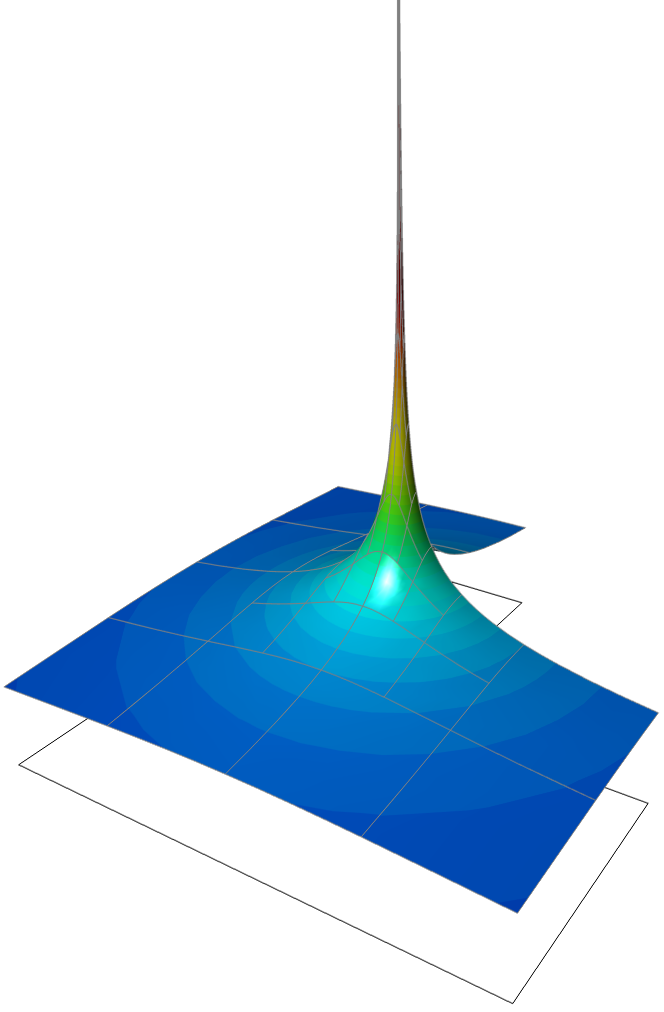
\includegraphics[width=0.75\textwidth]{img/title.png}
\end{center}

\vspace{-0.3cm}

{\Huge\bf Hermes2D}\\[6mm]
{\LARGE Tutorial}\\[2mm]
\hrule

\vspace{3mm}
{\Large Version 1.1 \hfill August 2009}



\newpage
\pagestyle{plain}


\setcounter{page}{1}
\pagestyle{plain}
\renewcommand{\thepage}{\roman{page}}
\tableofcontents
\newpage
\setcounter{page}{1}
\renewcommand{\thepage}{\arabic{page}}


\section{Introduction}
\label{ch:intro}

Welcome to Hermes2D, a free C++/Python library for rapid prototyping of adaptive FEM
and $hp$-FEM solvers for partial differential equations (PDE)
developed by an open source community around the $hp$-FEM group\footnote{\tt http://hpfem.org/}
at the University of Nevada, Reno. The library has a clean design and modular structure,
and it is available under the GPL license (Version 2, 1991). This document presents
a brief tutorial. Prior to reading the tutorial, install Hermes2D using instructions
on its home page. All tutorial examples can be found in the directory {\tt tutorial/}.

The $hp$-FEM is a modern version of the finite element method (FEM). It is capable of
extremely fast, exponential convergence through suitable adaptive combination of
elements of variable diameter $h$ and polynomial degree~$p$. Hermes2D is fully PDE-independent,
i.e., it does not contain any techniques which would work for a selected class of PDE only.
Approximations can be done using quality $H^1$, $\Hcurl$, $\Hdiv$, and $L^2$ conforming
higher-order elements (which can be combined in the discretization of multiphysics
problems via the novel adaptive multimesh $hp$-FEM if needed).

Here is a list of main points where Hermes differs from most other
$hp$-FEM and FEM codes:
\begin{itemize}
  \item {\em PDE-independent adaptivity algorithms \cite{miro}}. Hermes does not use any methods or algorithms
        that would restrict its applicability to some particular PDE type. In particular, adaptivity is
        guided by robust computational a-posteriori error estimates that work equally for any PDE.
  \item {\em Arbitrary-level hanging nodes \cite{socedo}}. Hermes is capable of handling arbitrarily irregular
        meshes. This means that extremely small elements can be adjacent to large ones. When an element
        is refined, its neighbors are never altered as in other adaptivity algorithms.
  \item {\em Monolithic multimesh $hp$-FEM discretization \cite{multimesh1}}. Different physical fields or
        solution components can be approximated on individual meshes. The approximation is
        monolithic, i.e., no error is caused by operator splitting, no error is caused by transferring data
        between different meshes.
  \item {\em Adaptive multimesh $hp$-FEM on dynamical meshes for time-dependent
        problems \cite{dusoce,sodukru}}. Different physical fields or
        solution components in time-dependent problems can be approximated
        on individual meshes that evolve in time independently of each other.
        The discretization of the PDE system is monolithic.
\end{itemize}
See the Hermes2D home page\footnote{\tt http://hpfem.org/main/hermes.php} for other interesting features.

\section{Tutorial}
\label{ch:tutorial}


This tutorial should give you a general idea of how to code applications with Hermes2D.
Note that there is an interactive graphical GUI Agros2D\footnote{http://hpfem.org/hermes2d/}
that allows you to use Hermes without programming, and an interactive web
notebook\footnote{http://nb.femhub.org/}
that allows you to use Hermes from any web browser without even installing it.
In addition to the tutorial examples, the directory {\tt examples/} contains a variety
of models that may help you to get started with your own applications.


%%%%%%%%%%%%%%%%%%%%%%%%%%%%%%%%%%%%%%%%%%%%%%%%%%%%%%%%%%%%%%%%%%%%%%%%%%%%%%%%%%%%%%%%%%%%%%%%%%%%

\subsection{Creating a Mesh}

Every finite element computation starts with partitioning of the problem domain
into simple elements. Here, we will be using triangles and quadrilaterals.
Normally this is done by specialized mesh generators, but in many cases we
can type the mesh file by hand, as shown below. This will also allow us to explain
concepts such as boundary markers. Moreover, thanks to the adaptive capabilities
of Hermes2D, you may find that in many cases you no longer need a mesh generator
and very fine meshes to obtain accurate results. All you need to do is partition
the domain very coarsely into several large elements.

Suppose we want to define an L-shaped domain with a rounded corner, as shown in
Figure~\ref{fig:simplemesh}.

\begin{figure}[ht]
  \smallskip\centering
  \includegraphics[width=0.52\textwidth]{img/simplemesh}
  \caption{Node and element numbering on an L-shaped domain.}
  \label{fig:simplemesh}
\end{figure}
The domain has already been partitioned into four large
elements, two quadrilaterals and two curvilinear triangles, each numbered from 0 to 3.
We also need to number all vertices of the mesh and assign markers to boundary edges.
These will be used later for creating boundary conditions.

Hermes2D uses a very simple mesh file format which we will use to describe the above
domain. You can find the complete mesh file here: {\tt hermes2d/tutorial/ 01-mesh/domain.mesh}.
The file consists of variable assignments. Each variable can hold a real number,
a list of real numbers or a list of lists. The following are all valid definitions
in the Hermes2D mesh file format:
\index{Mesh!file format}

\lstset{language=make}
\begin{lstlisting}
# comments start with a hash
var = 5.0 + cos(pi)  # number
list = { 1, 2, 3, 4, var }  # list
pairs = { {1, 2}, {1, var}, {0, list} }  # list of lists
\end{lstlisting}

The mesh file must contain at least these variables: {\tt vertices}, {\tt elements} and
{\tt boundaries}. The variable {\tt vertices} must supply a list of coordinates of the
mesh vertices and in our case it may look like this:

\begin{lstlisting}
a = 1.0  # size of the mesh
b = sqrt(2)/2

vertices =
{
  { 0, -a },    # vertex 0
  { a, -a },    # vertex 1
  { -a, 0 },    # vertex 2
  { 0, 0 },     # vertex 3
  { a, 0 },     # vertex 4
  { -a, a },    # vertex 5
  { 0, a },     # vertex 6
  { a*b, a*b }  # vertex 7
}
\end{lstlisting}

The variable {\tt elements} lists all elements in the mesh.
Elements are defined by the (zero-based) indices of their vertices in
counter-clockwise order, and an extra number, denoting the element marker.
Element markers can be used to distinguish areas of the domain with different
material parameters. If the domain consists of one material,
all elements can be assigned zero markers.
\index{Marker!element}

\begin{lstlisting}
elements =
{
  { 0, 1, 4, 3, 0 },  # quad 0
  { 3, 4, 7, 0 },     # tri 1
  { 3, 7, 6, 0 },     # tri 2
  { 2, 3, 6, 5, 0 }   # quad 3
}
\end{lstlisting}

\index{Marker!boundary}
The last mandatory variable, {\tt boundaries}, assigns boundary markers to
all boundary edges. By default, all edges have zero markers. Only those with
positive markers are considered to be part of the domain boundary and can be
assigned a boundary condition, as we will see later.
An edge is identified by two vertex indices.

\begin{lstlisting}
boundaries =
{
  { 0, 1, 1 },
  { 1, 4, 2 },
  { 3, 0, 4 },
  { 4, 7, 2 },
  { 7, 6, 2 },
  { 2, 3, 4 },
  { 6, 5, 2 },
  { 5, 2, 3 }
}
\end{lstlisting}

Finally, the file can also include the variable {\tt curves}, which lists all curved edges.
Each curved edge is described by one NURBS curve, defined by its degree, control points and
knot vector. Simplified syntax is available for circular arcs.

\index{NURBS}
A NURBS curve is defined by its degree, control points with weights and the knot
vector. The degree $d$ is a positive integer, usually 1, 2, 3 or 5. Lines and polylines
are of degree 1, circles have degree 2 and free-form curves are of degree 3 or 5.
The control points $p_i,\; i = 0 \dots n$, are the main tool for changing the shape of
the curve. A curve of degree $d$ must have at least $d+1$ control points. In Hermes2D,
the endpoints of the edge are always assumed to be the first and last control points
and therefore only the inner control points are listed in the mesh file.
All control points have an associated weight $w_i \geq 0$ which influences
the shape of the curve near the corresponding control point.
If $w_i = 0$ then $p_i$ has no effect on the shape.
As $w_i$ increases, the curve is pulled towards $p_i$. In the above definition of
the variable {\tt curves}, $points$ is a list of real-valued triples.

The knot vector is a sequence of $m+1$ values that determines how much and where the
control points influence the shape. The relation $m = n+d+1$ must hold. The sequence is
nondecreasing, $t_i \leq t_{i+1}$, and divides the whole interval $[0,1]$ into smaller
intervals which determine the area of influence of the control points. Since the curve
has to start and end at the edge vertices, the knot vector in Hermes2D always starts
with $d+1$ zeros and ends with $d+1$ ones. Only the inner knots are listed in the
above definition of the variable {\tt curves}, where $knots$ is a simple list of real values.

\index{NURBS}

\begin{lstlisting}
curves =
{
  { 4, 7, 45 },  # +45 degree circular arcs
  { 7, 6, 45 }
}
# EOF
\end{lstlisting}




%%%%%%%%%%%%%%%%%%%%%%%%%%%%%%%%%%%%%%%%%%%%%%%%%%%%%%%%%%%%%%%%%%%%%%%%%%%%%%%%%%%%%%%%%%%%%%%%%%%%

\subsection{Loading and Viewing a Mesh}

\index{Mesh!loading}
\index{Mesh!viewing}
Let us start with a ``Hello world'' example of using Hermes2D. We will load the mesh
we have just created and display it in a window.

\lstset{language=C++}
\begin{lstlisting}
#include "hermes2d.h"

int main(int argc, char* argv[])
{
  // load the mesh file
  Mesh mesh;
  mesh.load("domain.mesh");
\end{lstlisting}

First, an instance of the class {\tt Mesh} is created. If you are
a~C~programmer, you can think of a~class as a~{\tt struct} that also contains functions
(called methods in C++), that operate on the data members of the structure.
The class {\tt Mesh} contains the method {\tt load()}, which is used to load our mesh file.

\lstset{language=C++}
\begin{lstlisting}
  // perform some sample initial refinements
  mesh.refine_all_elements();          // refines all elements
  mesh.refine_towards_vertex(3, 4);    // refines mesh towards
                                       // vertex #3 (4x)
  mesh.refine_towards_boundary(2, 4);  // refines all elements
                                       // along boundary 2 (4x)
  mesh.refine_element(86, 0);          // refines element #86
                                       // isotropically
  mesh.refine_element(112, 0);         // refines element #112
                                       // isotropically
  mesh.refine_element(84, 2);          // refines element #84
                                       // anisotropically
  mesh.refine_element(114, 1);         // refines element #114
                                       //anisotropically
\end{lstlisting}

The portion of code above illustrates various types of initial mesh refinements.
It does not matter if the mesh becomes irregular, in fact, irregular
meshes are at the heart of Hermes.
%See Section~\ref{sec:meshmethods} for other ways of modifying meshes on the fly.
Other ways of modifying meshes on the fly include
\begin{verbatim}
Mesh::refine_element(int id, int refinement = 0)
Mesh::refine_by_criterion(int (*criterion)(Element* e), int depth)
Mesh::refine_towards_vertex(int vertex_id, int depth)
Mesh::regularize(int n)
Mesh::unrefine_element(int id)
Mesh::unrefine_all_elements()
\end{verbatim}
(see files {\tt mesh1.cpp} and {\tt mesh2.cpp} for details).

\lstset{language=C++}
\begin{lstlisting}
  // display the mesh
  // (100, 100) is the upper left corner position
  // 500 x 500 is the window size
  MeshView mview("Hello world!", 100, 100, 500, 500);
  mview.show(&mesh);
\end{lstlisting}
The above code illustrates how to visualize the mesh using the class {\tt MeshView}.
You can initialize it by supplying the title of the window and its initial position and size (all of these
parameters are optional). {\tt MeshView} provides the method {\tt show}, which
displays a window showing the mesh, see Figure~\ref{fig:meshview}.

\begin{figure}[h!]
  \centering\medskip
  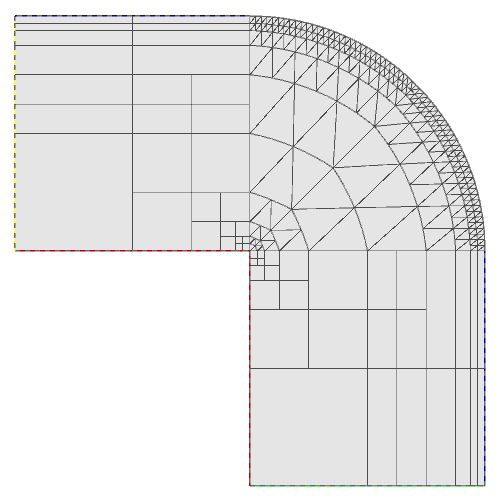
\includegraphics[width=0.52\textwidth]{img/meshview2.png}
  \caption{Image of the mesh created via the MeshView class.}
  \label{fig:meshview}
\end{figure}

\lstset{language=C++}
\begin{lstlisting}
  // wait for keyboard or mouse input
  View::wait();
  return 0;
}
\end{lstlisting}
At the end of the program, you may want to call the method {\tt View::wait()} to pause
the program, so that you have a chance to see its windows.

%%%%%%%%%%%%%%%%%%%%%%%%%%%%%%%%%%%%%%%%%%%%%%%%%%%%%%%%%%%%%%%%%%%%%%%%%%%%%%%%%%%%%%%%%%%%%%%%%%%%

\subsection{Setting up a Finite Element Space}

\index{Space!creating}
With the mesh definition in place we can start preparing the finite element calculation.
Hermes2D follows closely the mathematical concept of FEM in the
sense that you are required to construct a finite element space on top of a mesh
before performing any FE calculation. The following predefined spaces are currently
available:
\begin{itemize}
  \item {\tt H1Space} -- \index{Space!$H^1$} the most common space of continuous,
        piecewise-polynomial functions belonging to $H^1(\Omega) = \{ v \in L^2(\Omega);
        \nabla u \in (L^2(\Omega))^2 \}$,
  \item {\tt HcurlSpace} -- \index{Space!$\Hcurl$} the space of vector-valued functions discontinuous along mesh edges, with
        continuous tangential component on the edges $\bfH(\mbox{curl},\Omega) = \{ \bfE \in (L^2(\Omega))^2;
        \nabla \times \bfE \in L^2(\Omega)\}$,
  \item {\tt HdivSpace} -- \index{Space!$\Hdiv$} the space of vector-valued functions discontinuous along mesh edges, with
        continuous normal component on the edges $\bfH(\mbox{div},\Omega) = \{ \bfv \in (L^2(\Omega))^2;
        \nabla \cdot \bfv \in L^2(\Omega)\}$,
  \item {\tt L2Space} -- \index{Space!$L^2$} the space of functions discontinuous along mesh edges,
        belonging to the space $L^2(\Omega)$.
\end{itemize}

\index{Function!basis} \index{Function!edge} \index{Function!bubble}
All these spaces allow for higher-order elements and meshes with hanging nodes.
If you are not familiar with higher-order FEM, let us just say that the spaces can contain
quadratic, cubic, etc., {\em edge functions} that generate higher-degree
polynomials along mesh edges, and {\em bubble functions} that complete the higher-order
approximation in element interiors. An edge function is associated with a mesh edge,
a bubble function is associated with an element
(see Figure \ref{fig:basisfn}).

\begin{figure}[!ht]
  \centering\bigskip
  \includegraphics[width=\textwidth]{img/basisfn.jpg}
  \caption{\protect\centering Fourth-order edge function (left) and\break
  one of the fifth-order bubble functions (right).}
  \label{fig:basisfn}
\end{figure}

There are many possible ways of defining the
higher-order basis functions. A particular set of polynomials is called
\emph{shapeset}\index{Shapeset}. Using good shapeset is crucial for the
performance of the $hp$-FEM. No shapeset can be optimal for all possible operators.
Therefore, Hermes2D offers several shapesets from which
you need to choose when creating a FE space. The ones which perform best
in most computations (according to our experience) are simply called
{\tt H1Shapeset}, {\tt HcurlShapeset}, {\tt HdivShapeset} and {\tt L2Shapeset}.
Others can be found in the files {\tt shapeset\_*\_all.h}. A single shapeset
can be used for more than one space.

We are now ready for an example. The following code snippets come from
\verb"hermes2d/tutorial/02-space/main.cpp". We assume that a mesh has already
been loaded. First we create an instance of {\tt H1Shapeset} and then an
instance of {\tt H1Space}, supplying the mesh and shapeset pointers:

\begin{lstlisting}
 // create a shapeset and an H1 space
 H1Shapeset shapeset;
 H1Space space(&mesh, &shapeset);
\end{lstlisting}

After the space has been created, we need to initialize the polynomial
degrees\footnote{The words \emph{degree} and \emph{order} have the same meaning for us.}
of the elements. This can be done for individual elements by calling the method
\verb"Space::set_element_order()", or for all elements at once using
\verb"Space::set_uniform_order()". It is important to note that element degrees
are stored in the {\tt Space}, not in the {\tt Mesh}. The reason is that you can
have multiple different spaces with different element degrees over the same mesh.
In Hermes2D the mesh only stores geometrical information.

\begin{lstlisting}
 // assign element orders and initialize the space
 space.set_uniform_order(P_INIT);
 // enumerate basis functions
 space.assign_dofs();
\end{lstlisting}

A space created in this way is ready for use. By default, it is equipped with
zero Neumann boundary condition on the entire domain boundary. We will see
how to change that in Section \ref{sec:bc}.

\index{Space!viewing}
As a debugging feature, Hermes2D provides a visualization possibility for the
examination of all basis functions in a space. Similarly to {\tt MeshView},
you can create a {\tt BaseView} object and use it to display the basis of a space.
You can cycle through all basis functions in the window using the arrow keys.

\begin{lstlisting}
 // view the basis functions
 BaseView bview;
 bview.show(&space);
\end{lstlisting}

This is how Figure \ref{fig:basisfn} was obtained (press the ``{\tt 3}'' key for 3D mode).
You can experiment with element refinements and hanging nodes to see basis functions
on irregular meshes.

%More details on the space classes can be found in Section \ref{sec:space}.


%%%%%%%%%%%%%%%%%%%%%%%%%%%%%%%%%%%%%%%%%%%%%%%%%%%%%%%%%%%%%%%%%%%%%%%%%%%%%%%%%%%%%%%%%%%%%%%%%%%%

\subsection{Solving the Poisson Equation}
\label{sec:poisson}
\index{Poisson equation}

Let us solve the Poisson equation
\begin{equation} \label{poisson1}
-\Delta u = CONST_F
\end{equation}
on the L-shaped domain $\Omega$ from the previous example,
equipped with a homogeneous Dirichlet boundary condition
\begin{equation} \label{poisson2}
u = 0\ \ \  \mbox{on}\  \partial \Omega,
\end{equation}
where $CONST_F$ is a real number. The weak formulation \index{Weak formulation}
is derived in the standard way, first by multiplying equation (\ref{poisson1}) with a test
function $v$, then integrating over the domain $\Omega$, and then applying the Green's
theorem (integration by parts) to the second derivatives.
Because of the homogeneous Dirichlet condition
(\ref{poisson2}),
the proper space for the solution is $V = H^1_0(\Omega)$. The weak formulation reads:
Find $u \in V$ such that

\begin{equation} \label{poissonweak}
  \int_\Omega \nabla u \cdot \nabla v \;\mbox{d\bfx} = CONST_F \int_\Omega v \;\mbox{d\bfx}
\ \ \ \mbox{for all}\ v \in V.
\end{equation}
Equation (\ref{poissonweak}) has the standard form $a(u,v) = l(v)$ and thus in Hermes
we need a way to specify the bilinear form $a(u,v)$ and the linear form $l(v)$.
\index{Bilinear form} \index{Linear form}
In the code this is done by implementing the following two functions:

\begin{lstlisting}
scalar bilinear_form(RealFunction* fu, RealFunction* fv,
                     RefMap* ru, RefMap* rv);

scalar linear_form(RealFunction* fv, RefMap* rv);
\end{lstlisting}

These functions will be called for each element during the stiffness matrix
assembly and must return the values of the bilinear and linear forms for the given arguments.
{\tt RealFunction} represents one of the basis functions restricted to the
current element and {\tt RefMap} represents the reference mapping of the current element.
There are methods for extracting the values of the basis functions at integration points,
which allows you to evaluate the integrals by yourself, but this is normally not needed,
since many common weak forms have already been implemented.
In this case, we can simply use the predefined functions
\verb"int_grad_u_grad_v" and \verb"int_v":

\begin{lstlisting}
scalar bilinear_form(RealFunction* fu, RealFunction* fv,
                     RefMap* ru, RefMap* rv)
{
  return int_grad_u_grad_v(fu, fv, ru, rv);
}

scalar linear_form(RealFunction* fv, RefMap* rv)
{
  return CONST_F*int_v(fv, rv);
}
\end{lstlisting}


We can now state our problem in the following way
(taken from {\tt hermes2d/ tutorial/03-poisson}):

\begin{lstlisting}
 // initialize the weak formulation
 WeakForm wf(1); // num. eq.
 wf.add_biform(0, 0, bilinear_form);
 wf.add_liform(0, linear_form);
\end{lstlisting}
\index{WeakForm}

The class {\tt WeakForm} represents the weak formulation of the PDE and must be
initialized with the number of equations in the system, in our case one. We then
supply the class pointers to our bilinear and linear form functions. If the PDE
was more complicated, we could add multiple bilinear and/or linear forms. Last,
there are some integer numbers as arguments of {\tt add\_biform} and {\tt add\_liform}.
These are zeros if only one PDE is solved as in the present case. These integers will be
discussed in more detail in the context of PDE systems in Section \ref{sec:systems}.

Given the weak formulation and the discretization determined by the space and its mesh,
we can proceed to the approximate solution of the problem by the Galerkin method.
This method is the core of Hermes2D and provides a way to obtain a sparse linear
system of equations, represented by the class {\tt LinSystem} in the code. The solution
of the linear system then yields an approximate solution of the original problem.
\index{LinSystem}
\index{Galerkin method}

The class {\tt LinSystem} needs three things: your weak formulation, your spaces and
finally an external sparse matrix solver, for example CG or UMFPACK. The following lines
create the linear solver, initialize the {\tt LinSystem} class and pass a pointer to
the {\tt H1Space} we have created in the previous section.

\begin{lstlisting}
 // initialize the linear system and solver
 UmfpackSolver umfpack;
 LinSystem sys(&wf, &umfpack);
 sys.set_spaces(1, &space);
 sys.set_pss(1, &pss);
\end{lstlisting}

The last line must be included for historical reasons. During matrix assembly,
Hermes2D caches the values of all shape function polynomials for better performance.
The cache is represented by the class {\tt PrecalcShapeset} and you have to
include the following line at the beginning your program:

\begin{lstlisting}
 PrecalcShapeset pss(&shapeset);
\end{lstlisting}

Finally, we tell {\tt LinSystem} to assemble the stiffness matrix and the right-hand
side and solve the resulting linear system: \index{Stiffness matrix}

\begin{lstlisting}
 // assemble the stiffness matrix and solve the system
 Solution sln;
 sys.assemble();
 sys.solve(1, &sln);
\end{lstlisting}

The last two lines can be repeated many times in time-dependent problems. For
the Poisson problem, however,
we are finished. The instance of the class {\tt Solution}, upon the
completion of {\tt LinSystem::solve}, contains the approximate solution of
the PDE. You can ask for its values %, as described in Section \ref{sec:solution},
or you can visualize the solution immediately using the {\tt ScalarView} class:
\index{ScalarView}

\begin{lstlisting}
 // visualize the solution
 ScalarView view("Solution");
 view.show(&sln);
\end{lstlisting}

%Figure \ref{fig:poissoncomplete} lists the complete source code for this example.
For the complete source code we refer to the file {\tt tutorial/03-poisson/main.cpp}.
Figure \ref{fig:poisson} shows the output.

\begin{figure}[!ht]
  \centering\medskip
  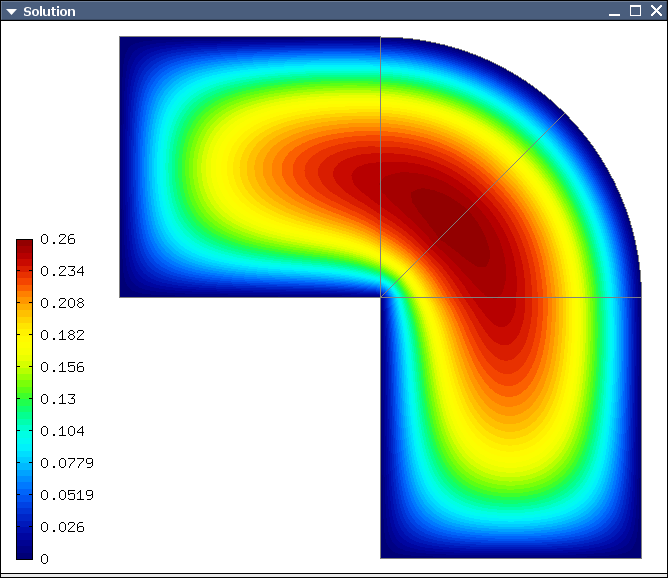
\includegraphics[width=0.75\textwidth]{img/poisson.png}
  \caption{Solution of the Poisson equation.}
  \label{fig:poisson}
\end{figure}



%\begin{figure}[p]
%  %\lstinputlisting{../examples/03-poisson/main.cpp}
%\begin{lstlisting}
%#include "hermes2d.h"
%#include "solver_umfpack.h"  // defines the class UmfpackSolver
%
%scalar bilinear_form(RealFunction* fu, RealFunction* fv,
%                     RefMap* ru, RefMap* rv)
%{
%  return int_grad_u_grad_v(fu, fv, ru, rv);
%}
%
%scalar linear_form(RealFunction* fv, RefMap* rv)
%{
%  return 2*int_v(fv, rv);
%}
%
%int main(int argc, char* argv[])
%{
%  Mesh mesh;
%  mesh.load("domain.mesh");
%  mesh.refine_element(0);
%
%  // initialize the shapeset and the cache
%  H1Shapeset shapeset;
%  PrecalcShapeset pss(&shapeset);
%
%  // create an H1 space
%  H1Space space(&mesh, &shapeset);
%  space.set_uniform_order(5);
%  space.assign_dofs();
%
%  // initialize the weak formulation
%  WeakForm wf(1);
%  wf.add_biform(0, 0, bilinear_form);
%  wf.add_liform(0, linear_form);
%
%  // initialize the linear system and solver
%  UmfpackSolver umfpack;
%  LinSystem sys(&wf, &umfpack);
%  sys.set_spaces(1, &space);
%  sys.set_pss(1, &pss);
%
%  // assemble the stiffness matrix and solve the system
%  Solution sln;
%  sys.assemble();
%  sys.solve(1, &sln);
%
%  // visualize the solution
%  ScalarView view("Solution");
%  view.show(&sln);
%  View::wait();
%  return 0;
%}
%\end{lstlisting}
%  \vspace{-2mm}
%  \caption{Complete listing of the Poisson equation example.}
%  \label{fig:poissoncomplete}
%\end{figure}


%%%%%%%%%%%%%%%%%%%%%%%%%%%%%%%%%%%%%%%%%%%%%%%%%%%%%%%%%%%%%%%%%%%%%%%%%%%%%%%%%%%%%%%%%%%%%%%%%%%%

\subsection{Adding Boundary Conditions}
\label{sec:bc}

\index{Boundary conditions!essential vs. natural}
Hermes2D recognizes two basic types of boundary conditions: {\em essential} and {\em natural}.
Essential boundary conditions influence and modify the finite element space while natural
conditions do not (they are incorporated into boundary integrals in the weak formulation).
In the context of elliptic problems, Dirichlet conditions are essential and Neumann/Newton
conditions are natural.

% -----------------------------------------------------------------------------------------

\subsubsection{Dirichlet Boundary Condition}

\index{Boundary conditions!Dirichlet}
Since essential conditions restrict degrees of freedom (DOF) in the FE space, 
they need to be incorporated while the space is set up.
The user has to provide the following two callback functions:

\begin{lstlisting}
int bc_types(int marker);
scalar bc_values(int marker, double x, double y);
\end{lstlisting}

The first one, given the boundary marker number, determines the type of BC which the associated
portion of the domain boundary belongs to, by returning one of the predefined constants 
\verb"BC_ESSENTIAL"
or \verb"BC_NATURAL". The second callback needs to return the boundary value for a given marker
and position on the boundary (only needed for essential boundary condition markers -- for natural
boundary conditions this value is ignored).
%(see Section \ref{sec:space} for more details and alternatives).
The space initialization might then look as follows:

\begin{lstlisting}
 H1Space space(&mesh, &shapeset);
 space.set_bc_types(bc_types);
 space.set_bc_values(bc_values);
\end{lstlisting}

Suppose we would like to modify the previous Poisson model problem in the following way:
$-\Delta u = CONST_F,\ u(x,y) = -\frac{CONST_F}{4}(x^2 + y^2)\,\ \mbox{on}\,\ \partial \Omega.$
Besides changing the linear form, we need to specify that all the boundary markers 1, 2, 3, 4
(refer to Figure \ref{fig:simplemesh} on page \pageref{fig:simplemesh}) denote the essential
boundary condition:

\begin{lstlisting}
int bc_types(int marker)
{
  return BC_ESSENTIAL;
}
\end{lstlisting}

Further, the value callback must return the value of the Dirichlet BC:

\begin{lstlisting}
scalar bc_values(int marker, double x, double y)
{
  return (-CONST_F/4)*(x*x + y*y);
}
\end{lstlisting}

It is easy to see that the solution to this problem is the function
$u(x,y) = -\frac{CONST_F}{4}(x^2 + y^2)$. For the value $CONST_F = -4$,
the output of example {\tt 04-bc-dirichlet} is shown
in Figure \ref{fig:dirichlet}.

\begin{figure}[!ht]
  \centering\medskip
  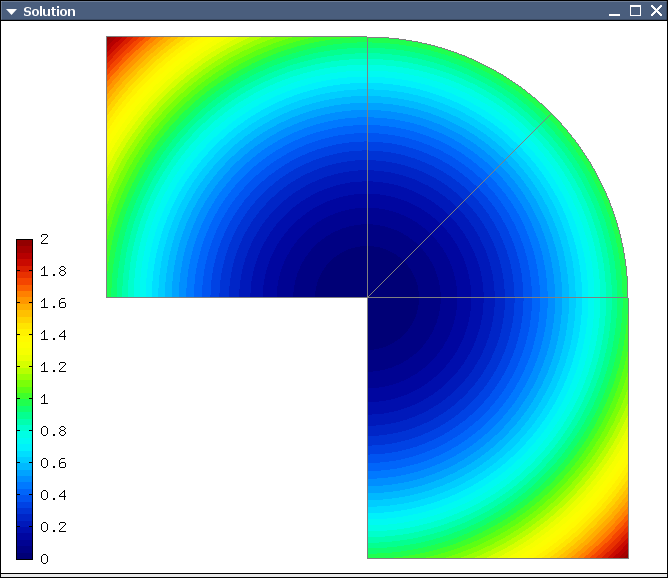
\includegraphics[width=0.7\textwidth]{img/dirichlet.png}
  \caption{Solution of the Dirichlet problem.}
  \label{fig:dirichlet}
\end{figure}

% -----------------------------------------------------------------------------------------

\subsubsection{Neumann Boundary Condition}

\index{Boundary conditions!Neumann}
Next, let us play with Neumann boundary conditions. The new model problem
will have the form
\begin{eqnarray*}
  -\Delta u = CONST_F,\ \ \ \ \ &&u = 0\,\ \mbox{on}\,\ \Gamma_4,\\
                           &&\dd{u}{n} = C_1\,\ \mbox{on}\,\ \Gamma_1,\\
                           &&\dd{u}{n} = C_2\,\ \mbox{on}\,\ \Gamma_2,\\
                           &&\dd{u}{n} = C_3\,\ \mbox{on}\,\ \Gamma_3.
\end{eqnarray*}
where $\Gamma_1 \dots \Gamma_4$ correspond to the edges marked $1 \dots 4$ in Figure
\ref{fig:simplemesh}. Now, the weak formulation contains some
surface integrals:
$$\int_\Omega \nabla u \cdot \nabla v \;\mbox{d\bfx} =
  CONST_F\int_\Omega v \;\mbox{d\bfx}
  + C_1\int_{\Gamma_1} \!v \;\mbox{d}l
  + C_2\int_{\Gamma_2} \!v \;\mbox{d}l
  + C_3\int_{\Gamma_3} \!v \;\mbox{d}l
$$

In Hermes2D, all forms in the standard weak formulation $a(u,v) = l(v)$
are in fact defined as a sum of contributions from volume integrals and from
surface integrals. In the case of the linear form $l(v)$, this means
$$l(v) = \sum_m l_m^{\,\rm vol}(v) + \sum_n l_n^{\,\rm surf}(v).$$
We have already seen volume linear forms in Section \ref{sec:poisson}.
Surface linear forms are implemented similarly. Our new right-hand side will
be represented by two functions with the following prototypes:

\begin{lstlisting}
scalar linear_form     (RealFunction* fv, RefMap* rv);
scalar linear_form_surf(RealFunction* fv, RefMap* rv,
                        EdgePos* ep);
\end{lstlisting}

and will be added to the {\tt WeakForm} by the following code:

\begin{lstlisting}
  // initialize the weak formulation
  WeakForm wf(1);
  wf.add_biform(0, 0, bilinear_form);
  wf.add_liform(0, linear_form);
  wf.add_liform_surf(0, linear_form_surf_Gamma_1, 1);
  wf.add_liform_surf(0, linear_form_surf_Gamma_2, 2);
  wf.add_liform_surf(0, linear_form_surf_Gamma_3, 3);
\end{lstlisting}

Note that the optional third argument to both {\tt add\_liform} and {\tt add\_liform\_ surf}
restricts the evaluation of the form to a given element or boundary marker.
For better readability, this is also reflected in the name of the form. The surface
linear forms are defined as follows:

\begin{lstlisting}
scalar linear_form_surf_Gamma_1(RealFunction* fv, RefMap* rv,
                                EdgePos* ep)
{
  return CONST_GAMMA_1 * surf_int_v(fv, rv, ep);
}

scalar linear_form_surf_Gamma_2(RealFunction* fv, RefMap* rv,
                                EdgePos* ep)
{
  return CONST_GAMMA_2 * surf_int_v(fv, rv, ep);
}

scalar linear_form_surf_Gamma_3(RealFunction* fv, RefMap* rv,
                                EdgePos* ep)
{
  return CONST_GAMMA_3 * surf_int_v(fv, rv, ep);
}
\end{lstlisting}

Here, we have used the predefined surface integral \verb"surf_int_v" (see the
file {\tt src/integrals\_h1.h}). If the boundary conditions were more complicated, we could also
have used \verb"surf_int_F_v", where {\tt F} stands for an arbitrary user-supplied
function returning the value $\partial u/\partial n$.

Passing marker number as the third argument to {\tt add\_liform} and others is
in fact a shortcut. In case the integration region is more complicated,
you need to define an area
% (see {\tt WeakForm::def\_area} in Section \ref{sec:weakform})
and pass its number.
The constant {\tt ANY} causes the form to be integrated over the whole domain
or its boundary and is the default value.

Refer to example {\tt 05-bc-neumann} for the complete code. Note that the mesh
is refined towards the re-entrant corner in order to capture the singular
gradient.

\begin{lstlisting}
  // load the mesh file
  Mesh mesh;
  mesh.load("domain.mesh");
  mesh.refine_towards_vertex(3, CORNER_REF_LEVEL);
\end{lstlisting}

The gradient magnitude can be visualized via a MagFilter:

\begin{lstlisting}
  // compute and show gradient magnitude
  // (note that the infinite gradient at the re-entrant
  // corner will be truncated for visualization purposes)
  ScalarView gradview("Gradient", 650, 0, 600, 600);
  MagFilter grad(&sln, &sln, FN_DX, FN_DY);
  gradview.show(&grad);
\end{lstlisting}

The approximate solution for the values $C_1 = -1/2$, $C_2 = 1$, $C_3 = -1/2$,
along with the singularity of gradient at the re-entrant corner are
shown in the following Figures \ref{fig:neumann2} and \ref{fig:neumann3}.

\begin{figure}[!ht]
  \centering\medskip
  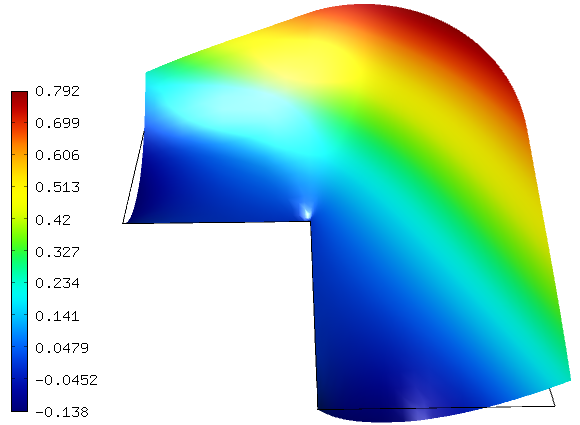
\includegraphics[width=0.7\textwidth]{img/neumann2.png}
  \caption{Solution of the Neumann problem.}
  \label{fig:neumann2}
\end{figure}

\begin{figure}[!ht]
  \centering\medskip
  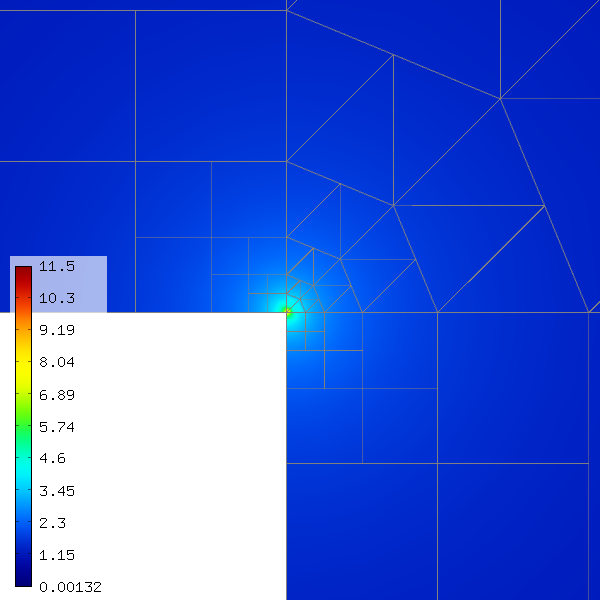
\includegraphics[width=0.7\textwidth]{img/neumann3.png}
  \caption{Detail of gradient singularity at the re-entrant corner.}
  \label{fig:neumann3}
\end{figure}



% -----------------------------------------------------------------------------------------

\subsubsection{Newton Boundary Condition}

\index{Boundary conditions!Newton}
\index{Boundary conditions!Robin}
Another common natural boundary condition is the Newton (sometimes called Robin) condition
of the form
$$\dd{u}{n} + c_1 u = c_2, \ \ \ \ c_1 \ne 0.$$
Analogously to Neumann conditions, also Newton conditions yield surface integrals. However,
this time they are both in the bilinear form and in the linear form,
The bilinear form is
a sum of volume and surface forms that can be added to the weak formulation using the methods
{\tt add\_biform} and {\tt add\_biform\_surf}. % (see Section \ref{sec:weakform}).
The surface bilinear form must have the following prototype:

\begin{lstlisting}
scalar bilinear_form_surf(RealFunction* fu, RealFunction* fv,
                          RefMap* ru, RefMap* rv, EdgePos* ep);
\end{lstlisting}

Inside this function you can use predefined
forms such as \verb"surf_int_u_v", \verb"surf_int_F_u_v"; (see the
file {\tt src/integrals\_h1.h}) or your custom forms.

Example {\tt 06-bc-newton} demonstrates typical usage of the Newton
boundary condition on a stationary heat transfer problem, where one part of the boundary
represents a heat exchange surface obeying the Newton law of cooling.
The following code snippet contains the linear and bilinear forms:

\begin{lstlisting}
scalar bilinear_form(RealFunction* fu, RealFunction* fv,
                     RefMap* ru, RefMap* rv)
  { return int_grad_u_grad_v(fu, fv, ru, rv); }

scalar bilinear_form_surf_Gamma_1(RealFunction* fu,
    RealFunction* fv, RefMap* ru, RefMap* rv, EdgePos* ep)
  { return H * surf_int_u_v(fu, fv, ru, rv, ep); }

scalar linear_form_surf_Gamma_1(RealFunction* fv,
                     RefMap* rv, EdgePos* ep)
  { return T0 * H * surf_int_v(fv, rv, ep); }
\end{lstlisting}

Here, $T_0$ is the exterior temperature, and $H$ is the heat flux.
The above forms are registered using

\begin{lstlisting}
  // initialize the weak formulation
  WeakForm wf(1);
  wf.add_biform(0, 0, bilinear_form);
  wf.add_biform_surf(0, 0, bilinear_form_surf_Gamma_1, 1);
  wf.add_liform_surf(0, linear_form_surf_Gamma_1, 1);
\end{lstlisting}

Figures \ref{fig:newton1} and \ref{fig:newton2} show the solution and
singularity of gradient at the re-entrant corner.

\begin{figure}[!ht]
  \centering\medskip
  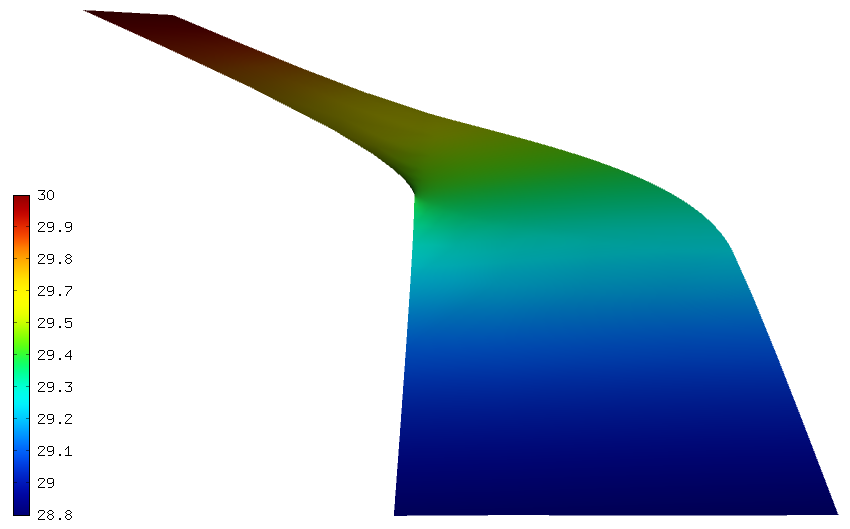
\includegraphics[width=0.7\textwidth]{img/newton1.png}
  \caption{Solution of the Newton problem.}
  \label{fig:newton1}
  \vspace{2mm}
\end{figure}

\begin{figure}[!ht]
  \centering\medskip
  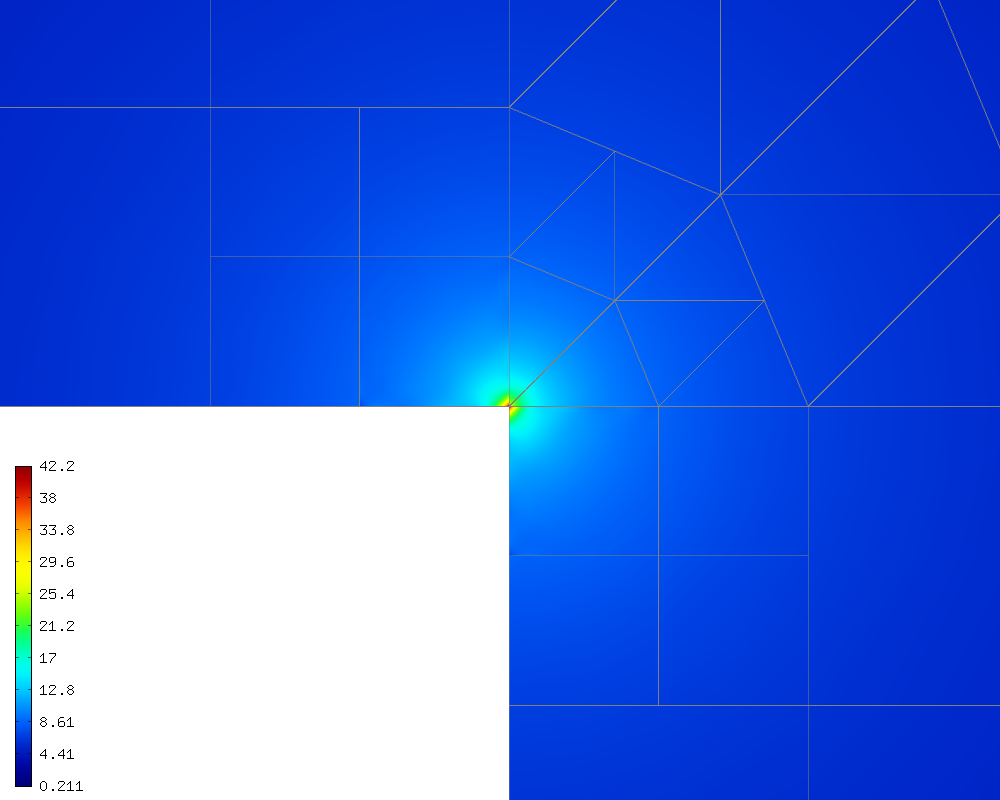
\includegraphics[width=0.7\textwidth]{img/newton2.png}
  \caption{Detail of gradient singularity at the re-entrant corner.}
  \label{fig:newton2}
\end{figure}



%%%%%%%%%%%%%%%%%%%%%%%%%%%%%%%%%%%%%%%%%%%%%%%%%%%%%%%%%%%%%%%%%%%%%%%%%%%%%%%%%%%%%%%%%%%%%%%%%%%%

\subsection{PDE Systems}
\label{sec:systems}

\index{Weak formulation}
\index{System of PDEs}

So far we have seen the solution of a single linear PDE with the weak formulation
of the form $a(u,v) = l(v)$, where $u, v$ were continuous approximations in the
$H^1$ space. Analogously one can handle equations whose solutions lie in the spaces
$\Hcurl$, $\Hdiv$ or $L^2$.

Moreover, Hermes2D can handle a system of $n$ linear
PDEs, provided that the weak formulation can be written as follows:
\begin{eqnarray}
  a_{11}(u_1,v_1)\,+ a_{12}(u_2,v_1)\,+ \cdots\,+ a_{1n}(u_n,v_1) &=& l_1(v_1), \nonumber \\
  a_{21}(u_1,v_2)\,+ a_{22}(u_2,v_2)\,+ \cdots\,+ a_{2n}(u_n,v_2) &=& l_2(v_2), \label{weaksystem} \\
                                                      &\vdots&     \nonumber  \\
  a_{n1}(u_1,v_n) + a_{n2}(u_2,v_n) + \cdots + a_{nn}(u_n,v_n) &=& l_n(v_n). \nonumber
\end{eqnarray}
The solution $\bfu = (u_1, u_2, \dots, u_n)$ and test functions $\bfv =
(v_1, v_2, \dots, v_n)$ belong to the space $W = V_1 \times V_2 \times \dots
\times V_n$, where each $V_i$ is one of the available function spaces.

Let us illustrate this by solving a simple problem of linear elasticity. Consider a
two-dimensional elastic body shown in Figure \ref{elastsample} (the bottom edge is
axis of planar symmetry).
In the plane-strain model of linear elasticity the goal is to determine the
deformation of the body subject to the forces $f$. The deformation is sought
as a vector function $u(x) = (u_1, u_2)^T$, describing the displacement of each point
$x \in \Omega$ after the load $f = (f_1, f_2)^T$ is applied.

\begin{figure}[!ht]
  \vspace{-2mm}
  \medskip\centering
  \includegraphics[width=0.87\textwidth]{img/elastsample}
  \caption{Geometry and boundary conditions.}
  \label{elastsample}
\end{figure}

The boundary conditions are
\begin{eqnarray}
  \dd{u_1}{n} &=&
  \begin{cases}
    f_1 & \text{on $\Gamma_3$,}\\
    0   & \text{on $\Gamma_2$, $\Gamma_4$, $\Gamma_5$}
  \end{cases}\label{elastbc1}
  \\
  \dd{u_2}{n} &=&
  \begin{cases}
    f_2 & \text{on $\Gamma_3$,}\\
    0   & \text{on $\Gamma_2$, $\Gamma_4$, $\Gamma_5$}
  \end{cases}\label{elastbc2}
  \\[2mm]
  u_1 &=& u_2 \ = \ 0 \ \ \mbox{on} \ \Gamma_1. \label{elastbc3}
\end{eqnarray}

Applying the standard procedure to the elastostatic equilibrium equations
(see \cite{lifshitz}), we arrive at the following weak formulation:
\begin{eqnarray*}
  \int_\Omega
    (2\mu\!+\!\lambda)\dd{u_1}{x_1}\dd{v_1}{x_1} + \mu\dd{u_1}{x_2}\dd{v_1}{x_2} +
    \mu\dd{u_2}{x_1}\dd{v_1}{x_2} + \lambda\dd{u_2}{x_2}\dd{v_1}{x_1}
    \,\mbox{d}\bfx \!\!&=&\!\!\!
    %\int_\Omega \rho f_1 v_1 \,\mbox{d}\bfx +
    \int_{\Gamma_3} \!\!f_1 v_1 \,\mbox{d}S, \\ \smallskip
  \int_\Omega
    \mu\dd{u_1}{x_2}\dd{v_2}{x_1} + \lambda\dd{u_1}{x_1}\dd{v_2}{x_2} +
    (2\mu\!+\!\lambda)\dd{u_2}{x_2}\dd{v_2}{x_2} + \mu\dd{u_2}{x_1}\dd{v_2}{x_1}
    \,\mbox{d}\bfx \!\!&=&\!\!\!
    %\int_\Omega \rho f_2 v_2 \,\mbox{d}\bfx +
    \int_{\Gamma_3} \!\!f_2 v_2 \,\mbox{d}S.
\end{eqnarray*}

We see that the weak formulation can indeed be written in the form (\ref{weaksystem}):
\begin{eqnarray}
  a_{11}(u_1, v_1) \!&=&\! \int_\Omega (2\mu+\lambda)\dd{u_1}{x_1}\dd{v_1}{x_1} + \mu\dd{u_1}{x_2}\dd{v_1}{x_2} \,\mbox{d}\bfx, \label{sysform1} \\
  a_{12}(u_2, v_1) \!&=&\! \int_\Omega \mu\dd{u_2}{x_1}\dd{v_1}{x_2} + \lambda\dd{u_2}{x_2}\dd{v_1}{x_1} \,\mbox{d}\bfx,\\
  a_{21}(u_1, v_2) \!&=&\! \int_\Omega \mu\dd{u_1}{x_2}\dd{v_2}{x_1} + \lambda\dd{u_1}{x_1}\dd{v_2}{x_2} \,\mbox{d}\bfx,\\
  a_{22}(u_2, v_2) \!&=&\! \int_\Omega (2\mu+\lambda)\dd{u_2}{x_2}\dd{v_2}{x_2} + \mu\dd{u_2}{x_1}\dd{v_2}{x_1} \,\mbox{d}\bfx, \label{sysform2} \\
  l_{1}(v_1) \!&=&\!
  %\int_\Omega \rho f_1 v_1 \,\mbox{d}\bfx +
  \int_{\Gamma_3} \!\!f_1 v_1 \,\mbox{d}S, \\
  l_{2}(v_2) \!&=&\!
  %\int_\Omega \rho f_2 v_2 \,\mbox{d}\bfx +
  \int_{\Gamma_3} \!\!f_2 v_2 \,\mbox{d}S.  \label{sysform3}
\end{eqnarray}

Here, $\mu$ and $\lambda$ are material constants (Lam\'e coefficients) defined as
$$\mu = \frac{E}{2(1+\nu)}, \ \ \ \ \  \lambda = \frac{E\nu}{(1+\nu)(1-2\nu)},$$
where $E$ is the Young modulus and $\nu$ the Poisson ratio of the material. For
steel, we have $E = 200$ GPa and $\nu = 0.3$. The load is $f = (0, 10^4)^T$ N.

The mesh for the problem, as well as the code which we will refer to below,
can be found in \verb"tutorial/07-system".

We will again start by defining the function spaces for the two solution
components, $u_1$ and $u_2$ (the $x$ and $y$ displacement). The boundary
conditions (\ref{elastbc1})--(\ref{elastbc3}) can be implemented as
\begin{lstlisting}
 int bc_types(int marker)
   { return (marker == 1) ? BC_ESSENTIAL : BC_NATURAL;; }

 int bc_values_x(int marker)
   { return 0;}

 double bc_values_y(EdgePos* ep)
   { return (ep->marker == 3) ? f : 0.0; }
\end{lstlisting}
Next we create the two displacement spaces,
{\tt xdisp} and {\tt ydisp}:
\begin{lstlisting}
 // create the x displacement space
 H1Space xdisp(&mesh, &shapeset);
 xdisp.set_bc_types(bc_types);
 xdisp.set_bc_values(bc_values_x);
 xdisp.set_uniform_order(P\_INIT);

 // create the y displacement space
 H1Space ydisp(&mesh, &shapeset);
 ydisp.set_bc_types(bc_types);
 ydisp.set_bc_values(bc_values_y);
 ydisp.set_uniform_order(P\_INIT);
\end{lstlisting}

Our {\tt WeakForm} instance will be initialized for two equations in the system.
After implementing the forms (\ref{sysform1})--(\ref{sysform2}) using the predefined integrals
{\tt int\_a\_dudx\_ dvdx\_b\_dudy\_dvdy} and {\tt int\_a\_dudx\_dvdy\_b\_dudy\_dvdx},
we can add them to the weak formulation using {\tt add\_biform}.
The first two parameters of this method correspond to the position of the form
in (\ref{weaksystem}) with zero-based numbering. Similarly for the surface linear form
(\ref{sysform3}).

\begin{lstlisting}
 // initialize the weak formulation
 WeakForm wf(2);
 wf.add_biform(0, 0, bilinear_form_0_0, SYM);
 wf.add_biform(0, 1, bilinear_form_0_1, SYM);
 wf.add_biform(1, 1, bilinear_form_1_1, SYM);
 wf.add_liform_surf(1, linear_form_1_surf);
\end{lstlisting}

An explanation of the extra parameter {\tt SYM} in {\tt add\_biform} is due.
Since the two diagonal forms $a_{11}$ and $a_{22}$ are symmetric, i.e.,
$a_{ii}(u,v) = a_{ii}(v,u)$, Hermes2D can be told to only evaluate them once for the
two cases $a_{ii}(u,v)$ and $a_{ii}(v,u)$ to speed up assembly. In fact, we should have
used the {\tt SYM} flag already in the previous sections, since the form
$a(u,v) = \nabla u \cdot \nabla v$ is also symmetric. This is however not the case
for all forms and the default value of the fourth parameter of {\tt add\_biform} is {\tt UNSYM}.

The off-diagonal forms $a_{12}(u_2, v_1)$ and $a_{21}(u_1, v_2)$ are not
(and cannot) be symmetric, since their arguments come from different spaces.
However, we can see that $a_{12}(u, v) = a_{21}(v, u)$, i.e., the corresponding blocks
of the local stiffness matrix are transposes of each other. Here, the {\tt SYM} flag
has a different effect: it tells Hermes2D to take the block of the local stiffness
matrix corresponding to the form $a_{12}$, transpose it and copy it where a block
corresponding to $a_{21}$ would belong, without evaluating $a_{21}$ at all (this is why
we don't add {\tt bilinear\_form\_1\_0}). This again speeds up the matrix assembly.
You can also use the flag {\tt ANTISYM}, which moreover inverts the sign of the block.
This makes sense in the case where $a_{ij}(u, v) = -a_{ji}(v, u)$.

It is recommended that you start with the default (and safe) {\tt UNSYM} flag for all
forms when developing your project, and only optimize the evaluation of the forms when
the code works well.

With the {\tt WeakForm} and spaces ready, we can initialize the linear system.
The only difference is that we now have two spaces determining the discretization
of the problem.

\begin{lstlisting}
 LinSystem sys(&wf, &umfpack);
 sys.set_spaces(2, &xdisp, &ydisp);
\end{lstlisting}

All that is left is to assemble the stiffness matrix and solve the system.
Since we have two equations and two spaces, we receive two solutions, one for each
displacement component:
\begin{lstlisting}
 Solution xsln, ysln;
 sys.assemble();
 sys.solve(2, &xsln, &ysln);
\end{lstlisting}

\smallskip As in the previous sections, it is now possible to visualize the displacement
solutions, e.g.,
\begin{lstlisting}
 ScalarView view("y displacement [m]");
 view.show(&ysln);
\end{lstlisting}
Usually, however, it is necessary to postprocess the solution in order to obtain more
informative visualization. In elasticity problems, one is often interested in material
stress, which is obtained by a formula combining the derivatives of the two displacements.
Hermes2D implements postprocessing through \emph{filters}. A filter is a special class
which takes up to three \verb"Solution"s, performs some computation and in the end acts
as another \verb"Solution", which can be visualized, or even fed into another filter.
Here, we can use the predefined filter \verb"VonMisesFilter", which calculates the
Von Mises stress:
\begin{lstlisting}
 VonMisesFilter stress(&xsln, &ysln, mu, lambda);
 view.show(&stress, EPS_HIGH, 0);
\end{lstlisting}
The second parameter of \verb"show" is the visualization accuracy and can be
\verb"EPS_LOW", \verb"EPS_NORMAL" (default) and \verb"EPS_HIGH". The third parameter is
the component number and is only valid for vector-valued (\Hcurl) solutions.

Finally, in elasticity problems, it may be illustrative to distort the computational
domain according to the calculated displacement. The function \verb"View::show" can be
passed three more optional parameters, which represent the $x$ and $y$ displacement
and a multiplier to make the displacements visible.
\begin{lstlisting}
 VonMisesFilter stress(&xsln, &ysln, mu, lambda);
 view.show(&stress, EPS_HIGH, 0, &xsln, &ysln, 1.5e5);
\end{lstlisting}

%The output of this code is shown in Figure \ref{elastsln}.

\clearpage

\begin{figure}[!ht]
  \medskip \centering
  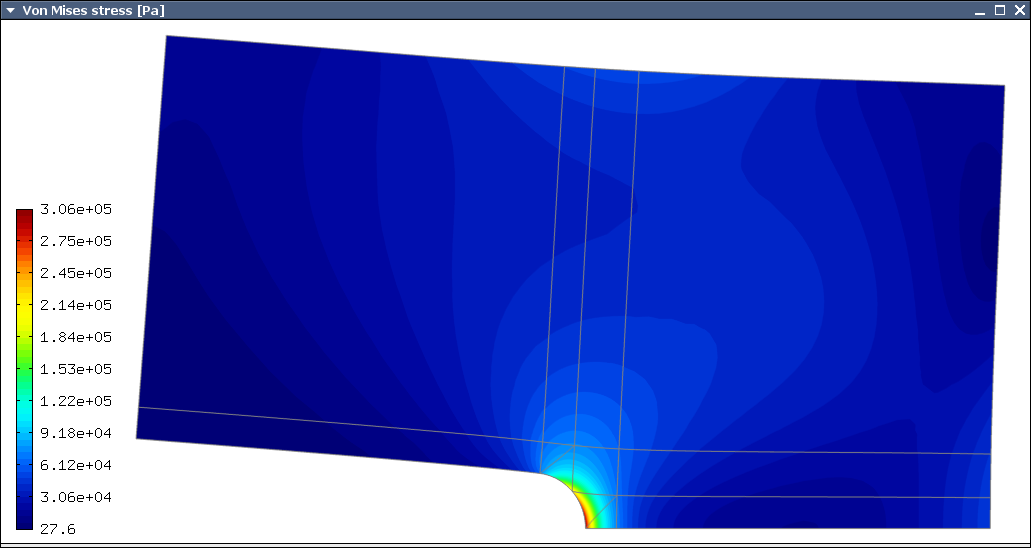
\includegraphics[width=\textwidth]{img/mises.png}
  \caption{Elastic stress plotted on deformed domain.}
  \label{elastsln}
\end{figure}


%%%%%%%%%%%%%%%%%%%%%%%%%%%%%%%%%%%%%%%%%%%%%%%%%%%%%%%%%%%%%%%%%%%%%%%%%%%%%%%%%%%%%%%%%%%%%%%%%%%%

\subsection{Time-Dependent Problems}

This section describes the implementation of a simple time-dependent
heat transfer model that can be found in {\tt tutorial/08-timedep}.
The model describes in a naive approximation how the St. Vitus cathedral
in Prague responds to changes in the surrounding air temperature
during one 24-hour cycle. The geometry is shown in Figure \ref{fig:vitus}.

We will solve the standard heat transfer equation
\begin{equation} \label{eqvit1}
c \varrho\frac{\partial T}{\partial t} - \lambda \Delta T = 0
\end{equation}
equipped with a Dirichlet condition
$$
T = T_{init}
$$
on the bottom edge $\Gamma_{ground}$ and a Newton condition
$$
\frac{\partial T}{\partial \nu} = \alpha(T_{ext}(t) - T)
$$
on the rest of the boundary $\Gamma_{air}$. Here, $c$ is the heat capacity of the material,
$\varrho$ the material density, $\lambda$ the thermal conductivity,
$T_{init}$ the fixed temperature on the
ground (same as the initial temperature of the building), and $\alpha$
the heat transfer coefficient \index{Initial condition}
between the building and the surrounding air. The surrounding air temperature
$T_{ext}$ is time-dependent of the form
$$
T_{ext}(t) = T_{init} + 10\sin(2\pi t/T_{final}),
$$
where $T_{final}$ is 24 hours (translated into seconds).

Equation (\ref{eqvit1}) is also equipped with an initial condition of the
form
$$
T(x,y,0) = T_{init}(x,y) \ \ \ \mbox{in} \ \Omega.
$$

\begin{figure}[!ht]
  \medskip \centering
  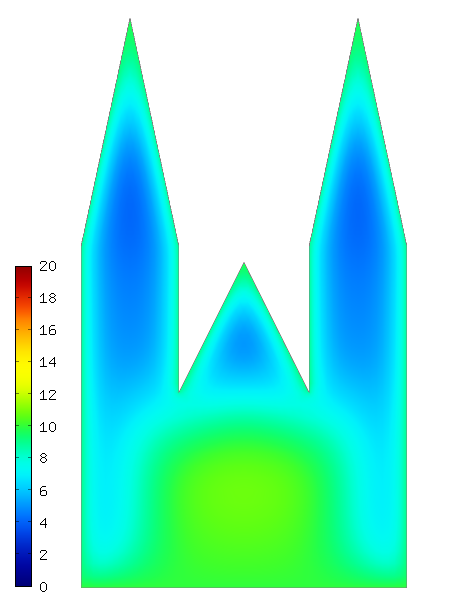
\includegraphics[width=0.6\textwidth]{img/vitus1.png}
  \caption{Model geometry and temperature distribution after 24 hours.}
  \label{fig:vitus}
\end{figure}

For simplicity we will use the implicit Euler method with a constant
time step $\tau$, which transforms equation (\ref{eqvit1}) into

$$
c \varrho\frac{T^{n+1} - T^n}{\tau} - \lambda \Delta T^{n+1} = 0.
$$
The corresponding weak formulation is
$$
\int_{\Omega} c \varrho\frac{T^{n+1}}{\tau} + \int_{\Omega} \lambda \nabla T^{n+1}\cdot \nabla v
+ \int_{\Gamma_{air}} \alpha \lambda T^{n+1}v = \int_{\Omega} c \varrho\frac{T^{n}}{\tau}
+ \int_{\Gamma_{air}} \alpha \lambda T_{ext}(t^{n+1})v.
$$
The implementation starts by defining the
boundary condition types
\begin{lstlisting}
int bc_types(int marker)
{
  if (marker == marker_ground) return BC_ESSENTIAL;
  else return BC_NATURAL;
}
\end{lstlisting}
and values
\begin{lstlisting}
scalar bc_values(int marker, double x, double y)
{
  if (marker == marker_ground) return T_INIT;
}
\end{lstlisting}
Then the space for the temperature $T$ is set up:
\begin{lstlisting}
  // set up spaces
  H1Space space(&mesh, &shapeset);
  space.set_bc_types(bc_types);
  space.set_bc_values(bc_values);
  space.set_uniform_order(P_INIT);
\end{lstlisting}

The bilinear and linear forms are defined as follows:
\begin{lstlisting}
// previous time step solution
Solution Tprev;

// volumetric forms
scalar bilinear_form_0_0_euler(RealFunction* fu, RealFunction* fv,
                               RefMap* ru, RefMap* rv)
{
  return HEATCAP * RHO * int_u_v(fu, fv, ru, rv) / TAU
    + LAMBDA * int_grad_u_grad_v(fu, fv, ru, rv);
}

scalar linear_form_0_euler(RealFunction* fv, RefMap* rv)
{
  return HEATCAP * RHO * int_u_v(&Tprev, fv, Tprev.get_refmap(),
                                 rv) / TAU;
}

// surface forms
scalar bilinear_form_0_0_surf(RealFunction* fu, RealFunction* fv,
                              RefMap* ru, RefMap* rv, EdgePos *ep)
{
  return LAMBDA * ALPHA * surf_int_u_v(fu, fv, ru, rv, ep);
}

scalar linear_form_0_surf(RealFunction* fv, RefMap* rv,
                          EdgePos *ep)
{
  return LAMBDA * ALPHA * temp_ext(TIME) * surf_int_v(fv, rv, ep);
}
\end{lstlisting}
These forms are registered as follows:
\begin{lstlisting}
  // weak formulation
  WeakForm wf(1);
  wf.add_biform(0, 0, bilinear_form_0_0_euler, UNSYM, ANY, 0);
  wf.add_liform(0, linear_form_0_euler, ANY, 1, &Tprev);
  wf.add_biform_surf(0, 0, bilinear_form_0_0_surf, ANY, 0,
                     marker_air);
  wf.add_liform_surf(0, linear_form_0_surf, ANY, 0, marker_air);
\end{lstlisting}

Before entering the main iteration loop, we need to initialize the previous solution
{\tt Tprev} with the initial condition $T_{init}$. \index{Initial condition}
Besides holding the finite element solution, the {\tt Solution} class
can be forced to return zero, to return a constant, or to return an arbitrary function
using the methods \verb"set_zero", \verb"set_const" and \verb"set_exact", respectively.
%(see Section \ref{sec:solution}).
Here we simply call \verb"set_const" and supply the initial temperature:
\begin{lstlisting}
  // set initial condition
  Tprev.set_const(&mesh, T_INIT);
\end{lstlisting}

We are now ready to start the iterative process. Since the stiffness matrix does
not depend on the solution, it only needs to be assembled once in the first time
step. For all remaining time steps it will be the same, and we just need to
re-construct the load vector. This is done via the Boolean variable {\tt rhsonly}
which is set to {\tt false} before the time stepping begins:
\begin{lstlisting}
  // assemble and solve
  ls.assemble(rhsonly);
  rhsonly = true;
  ls.solve(1, &Tnew);
\end{lstlisting}

At the end of each time step, the new solution must be stored for the next time step.
This is done by assigning {\tt Tnew} to {\tt Tprev}:
\begin{lstlisting}
  // copying the Tnew into Tprev
  Tprev = Tnew;
\end{lstlisting}
The assignment operator is overloaded for Solution and in fact is equal to calling
{\tt Solution::assign()}, which is an efficient way of handing over solution data from
one {\tt Solution} to another.

Another, more difficult time-dependent problem (nonlinear Navier-Stokes equations) is discussed
in Section \ref{sec:ns-timedep}.
%(see Section \ref{sec:solution}).

%%%%%%%%%%%%%%%%%%%%%%%%%%%%%%%%%%%%%%%%%%%%%%%%%%%%%%%%%%%%%%%%%%%%%%%%%%%%%%%%%%%%%%%%%%%%%%%%%%%%

\subsection{Some Remarks on Automatic Adaptivity}

In the computations that we carried out so far, we have not paid any attention
to the accuracy of the results. In general, a computation on a fixed mesh is
not likely to be very accurate. There is a need for {\it adaptive mesh refinement
(AMR)} algorithms that improve the quality of the approximation by refining
mesh elements where the approximation is bad.

In traditional low-order FEM, refining an element is not algorithmically complicated,
and so the most difficult part is to find out what elements should be
refined. To do this, people employ various techniques ranging from rigorous
guaranteed a-posteriori error estimates to heuristic criteria such as residual
error indicators, error indicators based on steep gradients, etc. Unfortunately,
none of these approaches is suitable for Hermes: The rigorous guaranteed error
estimates only exist for very simple problems, such as linear elliptic PDEs,
and thus they are far from PDE-independent. Heuristic techniques are not
employed in Hermes for the same reason, and moreover since such criteria
lack a transparent relation to the true approximation error.

Adaptive low-order FEM is known to be notoriously ineffcient, and practitioners
are rightfully skeptical of it. The reason is illustrated in Figure 13.

\begin{figure}[!ht]
  \medskip \centering
  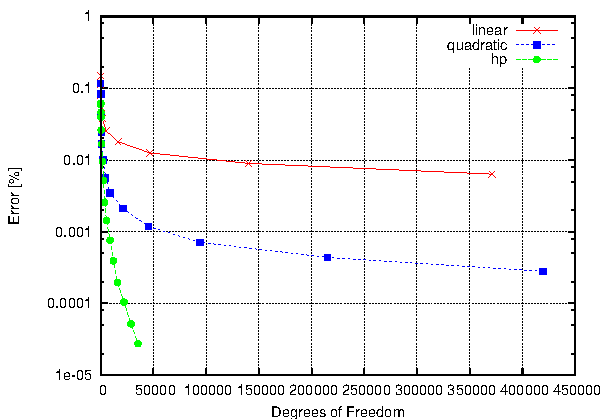
\includegraphics[width=0.8\textwidth]{img/conv_new}
  \caption{Typical convergence curves for adaptive linear FEM, quadratic
FEM, and $hp$-FEM.}
  \label{fig:conv}
\end{figure}

These convergence curves are typical representative examples, confirmed with
many numerical experiments of independent researchers, and supported with
theory. The horizontal axis shows (in linear scale) the number of degrees of freedom
(= size of the stiffness matrix) that increases during automatic adaptivity. The
vertical one shows the approximation error (in logarithmic scale). Note that in all
three cases, the error drops very fast during a short initial phase of the adaptive
computation. However, with both linear and quadratic FEM, the convergence slows
down dramatically as the adaptivity progresses. Note that the low-order FEM
is doomed to such slow convergence by its poor approximation properties ---
an excellent adaptivity algorithm cannot improve it (and a bad
algorithm can make it even worse).

In order to obtain fast, usable adaptivity (the green curve in Figure \ref{fig:conv}), one
has to resort to adaptive $hp$-FEM \cite{solin1}. The $hp$-FEM takes advantage of two
facts:

\begin{itemize}
\item Large high-degree elements approximate smooth parts of solution much
better than small linear ones. We created the example {\em smooth} to illustrate
this fact. Check it out, the results are impressive.
\item This holds the other way where the solution is not smooth.
\end{itemize}

Automatic adaptivity in the $hp$-FEM is substantially different from adaptivity
in low-order FEM, since every element can be refined in many different ways.
Figure \ref{fig:refinements} shows several example refinements for a fourth-order element.

\begin{figure}[!ht]
  \medskip \centering
  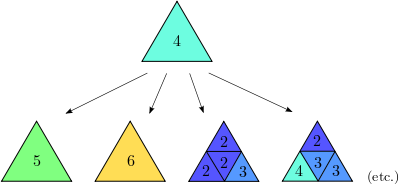
\includegraphics[width=0.9\textwidth]{img/refinements}
  \caption{Examples of $hp$-refinements.}
  \label{fig:refinements}
\end{figure}

Due to the large number of refinement options, classical error estimators (that
provide a constant error estimate per element) cannot be used to guide au\-
tomatic $hp$-adaptivity. For this, one needs to know the {\it shape} of the
approximation error.

In analogy to the most successful adaptive ODE solvers,
Hermes uses a pair of approximations with different orders of accuracy to obtain
this information: {\em coarse mesh solution} and {\em
fine mesh solution}. The initial coarse mesh is read from the mesh file,
and the initial fine mesh is created through its global refinement both in
{\it h} and {\it p}.
The fine mesh solution is the approximation of interest both during the adaptive
process and at the end of computation. The coarse mesh
solution represents its low-order part.

Both these solutions are evolved during the adaptive process
in a PDE-inde\-pen\-dent manner, based on the discrepancies between global and local
orthogonal projections. (Sometimes we replace the global orthogonal projection with
the solve on the coarse mesh, the difference is negligible.)

The obvious disadvantage of this approach to adaptivity is its higher computational cost,
especially in 3D. We are aware of this fact and would not mind at all replacing it with
some cheaper technique (that also is PDE-independent, works for elements of high orders,
and can be successfully used to guide $hp$-adaptivity).

\subsection{Adaptivity Example -- Electrostatic Micromotor}

Let us demostrate the use of automatic $hp$-adaptivity in Hermes2D on a linear elliptic problem
({\tt tutorial/09-adapt}) concerned with the calculation of
the electrostatic potential in the vicinity of the electrodes of an electrostatic
micromotor. This is a MEMS device free of any coils, and thus resistive to
strong electromagnetic waves (as opposed to classical electromotors).
Figure \ref{fig:micromotor} shows one half of the domain $\Omega$
(dimensions need to be scaled with $10^{-5}$ and are in meters).

\begin{figure}[!ht]
  \medskip \centering
  \includegraphics[width=0.85\textwidth]{img/micromotor}
  \caption{Computational domain for the micromotor problem.}
  \label{fig:micromotor}
\end{figure}

The subdomain $\Omega_2$ represents the moving part of the domain and the area bounded by $\Gamma_2$
represents the electrodes that are fixed. The distribution of the electrostatic potential $\varphi$ is governed by the equation
$$-\nabla\cdot\left(\epsilon_r\nabla\varphi\right) = 0,$$
equipped with the Dirichlet boundary conditions
$$\varphi = 0 V \ \ \ \ \ \mbox{on}\ \Gamma_1,$$
$$\varphi = 50 V \ \ \ \ \mbox{on}\ \Gamma_2.$$
The relative permittivity $\epsilon_r$ is piecewise-constant, $\epsilon_r = 1$ in $\Omega_1$ and
$\epsilon_r = 10$ in $\Omega_2$. The weak formulation reads
$$\int_\Omega \epsilon_r \nabla u \cdot \nabla v \dx = 0.$$
The varying parameter $\epsilon_r$ is handled by defining two bilinear forms in the code, one for
$\Omega_1$ and the other for $\Omega_2$. These two areas are delimited by element markers 1 and 2 in
the mesh, and the two forms are assigned to the corresponding markers during the registration of
the forms:
\begin{lstlisting}
 WeakForm wf(1);
 wf.add_biform(0, 0, biform1, SYM, 1);
 wf.add_biform(0, 0, biform2, SYM, 2);
\end{lstlisting}

The principal part of the example is the main adaptivity loop. In each iteration, the coarse problem
is solved first:
\begin{lstlisting}
 // solve the coarse problem
 LinSystem ls(&wf, &solver);
 ls.set_spaces(1, &space);
 ls.set_pss(1, &pss);
 ls.assemble();
 ls.solve(1, &sln);
\end{lstlisting}

Next, the reference solution must be obtained, which can be done by creating a refined copy of the mesh,
defining a temporary space with increased element orders and by assembling and solving an extra
linear system. However, for most problems, this can be automated using the class {\tt RefSystem}, which
handles all the temporary reference meshes and spaces transparently. All it needs is a pointer to our coarse
{\tt LinSystem}. The calculation of the reference solution is as simple as the following:
\begin{lstlisting}
 // solve the fine mesh problem
 RefSystem rs(&ls);
 rs.assemble();
 rs.solve(1, &sln_fine);
\end{lstlisting}

In the third and last step of each iteration, we refine our mesh and polynomial degrees stored
in our space using a class called {\tt H1OrthoHP}. This class offers two services: it is able to
calculate  the estimate of the overall error of the coarse solution in $H^1$ norm, and if the
error is too large, you can ask the class to $hp$-adapt your mesh and element orders optimally.

{\tt H1OrthoHP} is initialized with the number of spaces in the problem and pointers to them.
The method \verb"calc_error" takes pointers to the coarse and reference solutions and returns
$$e = \frac{|| u - u_{ref} ||_{H^1}}{|| u_{ref} ||_{H^1}}.$$
In the code this looks as follows:
\begin{lstlisting}
 H1OrthoHP hp(1, &space);
 double err_est = hp.calc_error(&sln_coarse, &sln_fine) * 100;
\end{lstlisting}

Finally, if {\tt err\_est} is still above the threshold {\tt ERR\_STOP}, we perform one
adaptivity step:

\begin{lstlisting}
 if (err_est < ERR_STOP) done = true;
 else {
   hp.adapt(THRESHOLD, STRATEGY, ADAPT_TYPE, ISO_ONLY, MESH_REGULARITY);
   ndofs = space.assign_dofs();
   if (ndofs >= NDOF_STOP) done = true;
 }
\end{lstlisting}

The parameters {\tt THRESHOLD}, {\tt STRATEGY}, {\tt ADAPT\_TYPE}, {\tt ISO\_ONLY}, {\tt MESH\_REGULARI\break TY}
have the following meaning: {\tt STRATEGY} indicates which adaptive strategy we
want to use.
\begin{itemize}
\vskip -5mm
\item {\tt STRATEGY == 0}: Refine elements until {\tt sqrt(THRESHOLD)} times total error
is processed. If more elements have similar error refine all to keep the mesh symmetric.
\item {\tt STRATEGY == 1}: Refine all elements whose error is bigger than {\tt THRESHOLD}
times maximum element error.
\item {\tt STRATEGY == 2}: Refine all elements whose error is bigger than {\tt THRESHOLD}.
\end{itemize}

If {\tt ADAPT\_TYPE == 0}, $hp$-adaptivity is performed (default). If {\tt ADAPT\_TYPE == 1},
the algorithm does $h$-adaptivity (fixed polynomial degrees of elements). This option is there
for comparison purposes. With {\tt ADAPT\_TYPE == 2} the algorithm does pure $p$-adaptivity (element
geometries fixed). This option
is there for completeness, adaptive $p$-FEM is not useful in practice.

The parameter {\tt ISO\_ONLY} determines whether quadrilateral elements
can be split anisotropically (into two elements). The parameter {\tt MESH\_REGULA\break RITY}
specifies maximum allowed level of hanging nodes: {\tt -1} means arbitrary-level
hanging nodes (default), and {\tt 1, 2, 3, ... } means 1-irregular mesh,
2-irregular mesh, etc. Hermes does not support adaptivity on regular meshes
because of its extremely poor performance.

It is a very good idea to spend some time playing with these parameters to
get a feeling for adaptive $hp$-FEM. Also look at other adaptivity examples in
the {\tt examples/} directory: {\tt layer}, {\tt lshape} deal with elliptic problems and have
known exact solutions. So do examples {\tt screen}, {\tt bessel} for time-harmonic
Maxwell's equations. These examples allow you to compare the error estimates
computed by Hermes with the true error. Examples {\tt crack}, {\tt singpert} show
how to handle cracks and singularly perturbed problems, respectively. There
are also more advanced examples illustrating automatic adaptivity for nonlinear
problems solved via the Newton's method, adaptive multimesh \hbox{$hp$-FEM},
adaptivity for time-dependent problems on dynamical meshes, etc.

But let's return to the micromotor example for a moment again: The computation
starts with a very coarse mesh consisting of a few quadrilaterals, some
of which are moreover very ill-shaped. Thanks to the anisotropic refinement
capabilities of {\tt H1OrthoHP}, the mesh quickly adapts to the solution (Figure \ref{fig:motor-sln})
and elements of reasonable shape are created near singularities, which occur
at the corners of the electrode (Figure \ref{fig:motor-grad}). Initially, all elements of the mesh
are of a low degree, but as the hp-adaptive process progresses, the elements
receive different polynomial degrees, depending on the local smoothness of the
solution (Figure \ref{fig:motor-orders}).

The gradient in Figure \ref{fig:motor-grad} was visualized using {\tt VectorView}. We have
seen this in the previous section. We plug in the same solution for both vector
components, but specify that its derivatives should be used:
\begin{lstlisting}
 gview.show(&sln, &sln, EPS_NORMAL, FN_DX_0, FN_DY_0);
\end{lstlisting}


\begin{figure}[!ht]
  \medskip \centering
  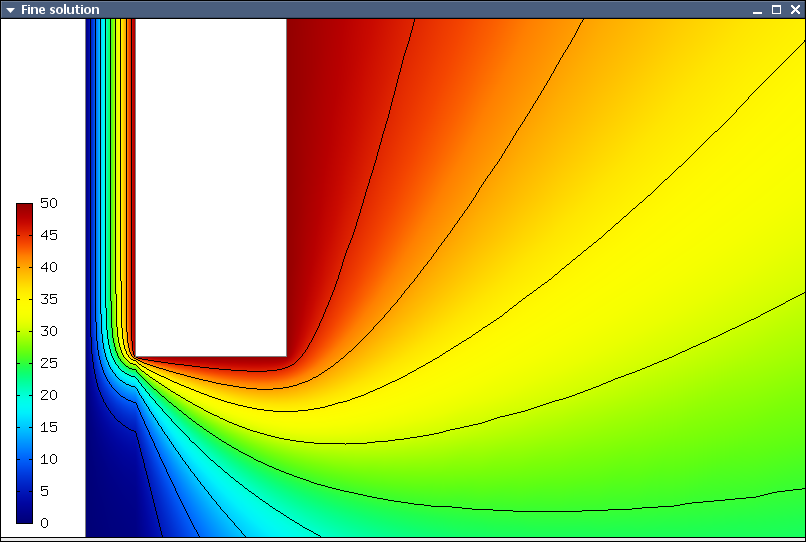
\includegraphics[width=0.8\textwidth]{img/motor-sln.png}
  \caption{Solution -- electrostatic potential $\varphi$ (zoomed).}
  \label{fig:motor-sln}
\end{figure}

\begin{figure}[!ht]
  \medskip \centering
  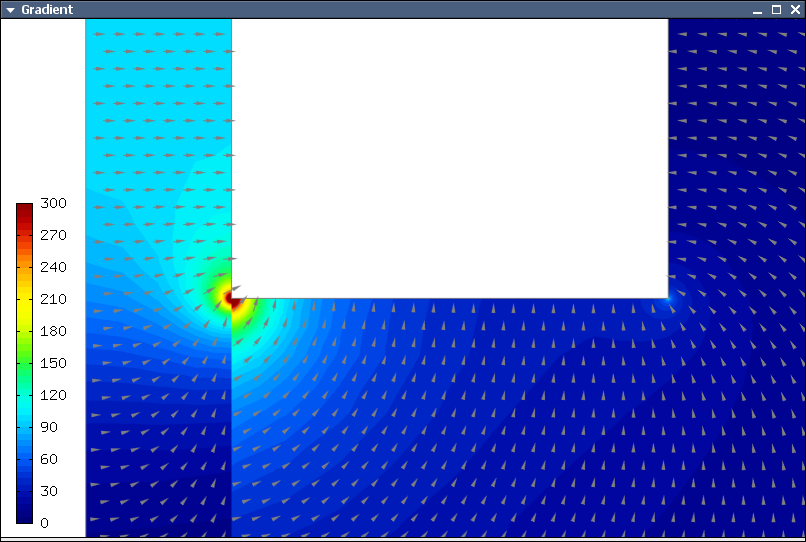
\includegraphics[width=0.8\textwidth]{img/motor-grad.png}
  \caption{Gradient of the solution $\bfE = -\nabla\varphi$ and its magnitude (zoomed).}
  \label{fig:motor-grad}
\end{figure}

\begin{figure}[!t]
  \medskip \centering
  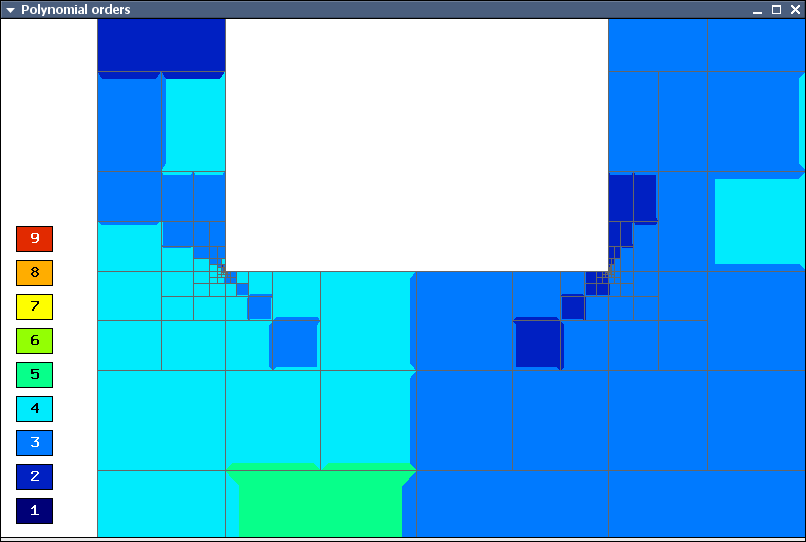
\includegraphics[width=0.8\textwidth]{img/motor-orders.png}
  \caption{Polynomial orders of elements near singularities (zoomed).}
  \label{fig:motor-orders}
  \vskip 5mm
\end{figure}

%%%%%%%%%%%%%%%%%%%%%%%%%%%%%%%%%%%%%%%%%%%%%%%%%%%%%%%%%%%%%%%%%%%%%%%%%%%%%%%%%%%%%%%%%%%%%%%%%%%%

\subsection{Adaptivity for PDE Systems}

The procedure described in the previous section could be extended directly to
systems of PDEs. In other words, two spaces can be passed into {\tt H1OrthoHP},
four solutions (two coarse, two reference) can be passed into {\tt calc\_error\_2},
and finally, adapt can be called as before. In this way, error estimates in
$H^1$ norm are calculated for elements in both spaces independently and the
worst ones are refined. However, this approach is not optimal if the PDEs are
coupled, since an error caused in one solution component influences the errors
in other components and vice versa.

Recall that in elliptic problems the bilinear form $a(u,v)$ defines the energetic inner product,
$$(u,v)_e = a(u,v).$$
The norm induced by this product,
$$||u||_e = \sqrt{(u,u)_e},$$
is called the {\it energy norm}. \index{Energy norm} \index{Norm!energy}
When measuring the error in the energy norm
of the entire system, one can reduce the above-mentioned difficulties dramatically.
When calculating the error on an element, the energy norm accounts
also for the error caused by other solution components.

Let us consider again the equations of linear elasticity from Section \ref{sec:systems}, but
now we will view them as a coupled PDE system.
Our domain (Figure \ref{fig:bracket}) is a bracket loaded on its top edge and fixed to a wall:
\begin{eqnarray*}
  \bfu \!&=&\! 0 \ \ \ \ \ \rm{on}\ \Gamma_1  \\
  \dd{u_2}{n} \!&=&\! f \ \ \ \ \ \rm{on}\ \Gamma_2 \\
  \dd{u_1}{n} = \dd{u_2}{n} \!&=&\! 0 \ \ \ \ \ \rm{elsewhere.}
\end{eqnarray*}
The dimensions are L = 0.7 m, T = 0.1 m and the force $f = 10^3$ N.

\begin{figure}[!ht]
  \medskip \centering
  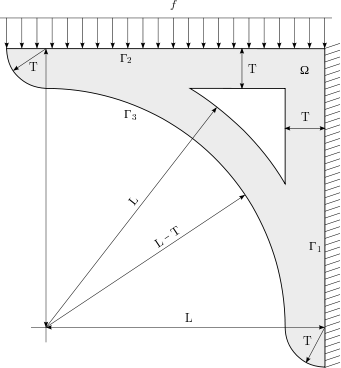
\includegraphics[width=0.55\textwidth]{img/bracket}
  \vspace{-2mm}
  \caption{Computational domain for the elastic bracket problem.}
  \label{fig:bracket}
\end{figure}

The implementation (see {\tt tutorial/10-adapt-system}) is very similar to the micromotor
example from the previous section. Again, the coarse and reference solutions are calculated
in the main loop, only this time we have two equations in the system, two meshes, two spaces, etc.
The only substantial difference is in the calculation of the error estimate. Instead of
\verb"calc_error()" we use the method \verb"calc_energy_error()", also a member of the
class \verb"H1OrthoHP":

\begin{lstlisting}
 H1OrthoHP hp(2, &xdisp, &ydisp);
 error = hp.calc_energy_error_2(&xsln, &ysln, &xrsln, &yrsln,
                    bilinear_form_0_0, bilinear_form_0_1,
                    bilinear_form_1_0, bilinear_form_1_1) * 100;
\end{lstlisting}

The arguments of \verb"calc_energy_error()" are: $n$ coarse solutions, $n$ reference solutions,
and finally $n \times n$ pointers to bilinear forms of the problem (row after row), which are used
for the calculation of the energy norm of the error.

(The function \verb"calc_energy_error_2()" used above is a type-safe wrapper for the
more general function \verb"calc_energy_error()", which takes a variable number of arguments.
%, see Section \ref{sec:calc_energy_norm}).

\begin{figure}[!ht]
  \medskip \centering
  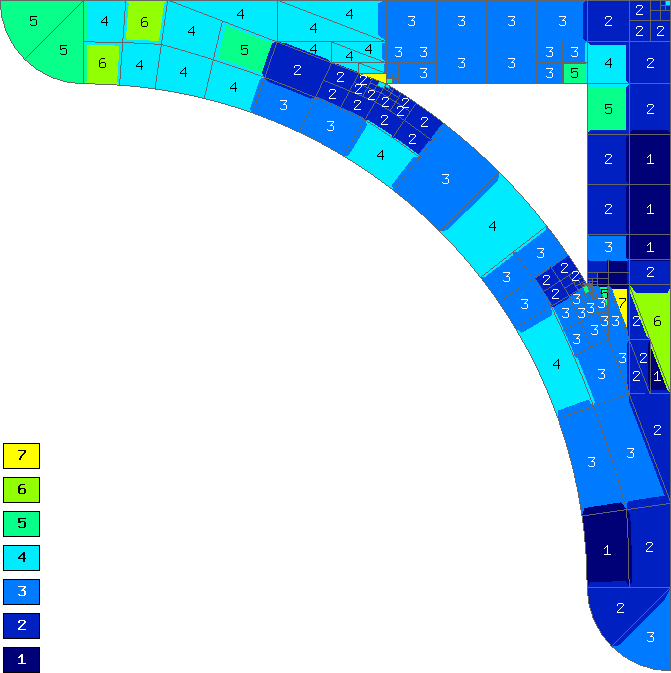
\includegraphics[height=0.5\textwidth]{img/sys-xorders.png}
  \caption{$x$ displacement -- mesh and polynomial degrees.}
  \label{fig:sys-xorders}
\end{figure}

\begin{figure}[!ht]
  \medskip \centering
  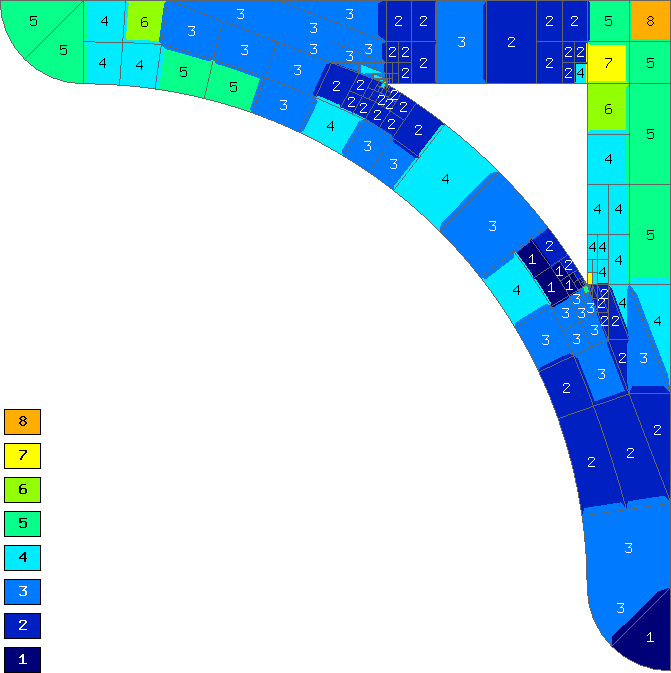
\includegraphics[height=0.5\textwidth]{img/sys-yorders.png}
  \caption{$y$ displacement -- mesh and polynomial degrees.}
  \label{fig:sys-yorders}
\end{figure}

Figures \ref{fig:sys-xorders} and \ref{fig:sys-yorders} show the two meshes and their polynomial
degrees after several adaptive steps. Note that they are slightly different, not only in
polynomial degrees, but also in element refinements. This is possible in Hermes2D thanks to
a technique called multi-mesh assembling
% (see Section \ref{sec:multimesh}),
which allows
all components of the solution to adapt independently. In problems whose components exhibit
substantially different behavior, one may even obtain completely different meshes.
See example {\tt multimesh} for a more advanced application of
multimesh $hp$-FEM to thermoelasticity.

%%%%%%%%%%%%%%%%%%%%%%%%%%%%%%%%%%%%%%%%%%%%%%%%%%%%%%%%%%%%%%%%%%%%%%%%%%%%%%%%%%%%%%%%%%%%%%%%%%%%

\subsection{Example ns-timedep}\label{sec:ns-timedep}

This model problem is concerned with the approximate solution of external
flow past a cylinder with unit diameter, as shown in Figure \ref{cylinderdomain}.

\begin{figure}[!ht]
  \medskip \centering
  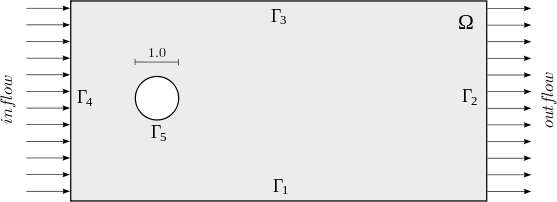
\includegraphics[width=0.95\textwidth]{img/cylinder}
  \caption{Domain for the Navier-Stokes problem.}
  \label{cylinderdomain}
\end{figure}

The motion of the fluid is described by the dimensionless incompressible
Navier-Stokes equations,
\begin{equation} \label{ns1}
  \dd{\bfu}{t} - \frac{1}{\rm Re} \Delta \bfu + (\bfu \cdot \nabla) \bfu + \nabla p  = 0,
\end{equation}
\begin{equation} \label{ns2}
  \nabla \cdot \bfu = 0,
\end{equation}
where $\bfu = (u_1, u_2)^T$ is the fluid velocity, $p$ is the kinematic pressure and Re
is the Reynods number. One way to solve the nonlinear system (\ref{ns1})--(\ref{ns2}) is to
introduce a small time step $\tau > 0$, replace the time derivative by a backward
difference formula and linearize the convective term
$(\bfu \cdot \nabla) \bfu \approx (\bfu^{n-1} \cdot \nabla) \bfu^n$, where $\bfu^n$ is the
approximate solution on the $n$-th time level. This leads to a system of linear PDEs for the
$n$-th time level
\begin{equation} \label{ns3}
  \frac{\bfu^n - \bfu^{n-1}}{\tau} - \frac{1}{\rm Re} \Delta \bfu^n +
    (\bfu^{n-1} \cdot \nabla) \bfu^n + \nabla p  = 0,
\end{equation}
\begin{equation} \label{ns4}
  \nabla \cdot \bfu^n = 0,
\end{equation}
Testing (\ref{ns3}) by the velocity test functions $(v_1, v_2)$ and testing (\ref{ns4})
by the pressure test function $q$, we obtain the following weak formulation:
$$\int_\Omega \frac{u_1 v_1}{\tau} +
  \frac{1}{\rm Re} \nabla u_1 \cdot \nabla v_1 +
  (\bfu^{n-1} \cdot \nabla) u_1 v_1 - p \dd{v_1}{x} \dx
  = \int_\Omega \frac{u^{n-1}_1 v_1}{\tau} $$
$$\int_\Omega \frac{u_2 v_2}{\tau} +
  \frac{1}{\rm Re} \nabla u_2 \cdot \nabla v_2 +
  (\bfu^{n-1} \cdot \nabla) u_2 v_2 - p \dd{v_2}{y} \dx
  = \int_\Omega \frac{u^{n-1}_2 v_2}{\tau} $$
$$\int_\Omega \dd{u_1}{x} q + \dd{u_2}{y} q \dx = 0 $$

The boundary and initial conditions \index{Initial condition} for the problem are
$$\bfu(\bfx, t) = (1, 0)^T \ \ \ \ \mbox{on}\ \ \Gamma_1 \cup \Gamma_3 \cup \Gamma_4$$
$$\bfu(\bfx, t) = (0, 0)^T \ \ \ \ \mbox{on}\ \ \Gamma_5$$
$$\mbox{\it ``do-nothing"}\ \ \ \ \mbox{on}\ \ \Gamma_2$$
\begin{equation} \bfu(\bfx, 0) = \bfu^0 = (0, 0)^T \label{ns:initial} \end{equation}

In CFD, the {\it do-nothing} condition is a common artificial boundary condition defining
an outlet for the fluid. It means that there is no restriction on the value
of the velocity on $\Gamma_2$.

The implementation starts by defining three spaces {\tt xvel}, {\tt yvel} and {\tt press}
for the three solution components $u_1$, $u_2$ and $p$. Using {\tt Space::set\_bc\_type}
we denote the Dirichlet boundary for velocity:
\begin{lstlisting}
 int xvel_bc_type(int marker)
   { return (marker != 2) ? BC_ESSENTIAL : BC_NONE; }
\end{lstlisting}
Returning {\tt BC\_NONE} for some part of the boundary assigns degrees of freedom but turns
off all surface integral processing on that part of the boundary, which is what we need
in this case.

Next we rewrite the weak formulation so that it fits into the block form (\ref{weaksystem})
on page \pageref{weaksystem}:
\begin{eqnarray*}
  a_{11}(u_1, v_1) &=& \int_\Omega \frac{u_1 v_1}{\tau} \dx +
                       \int_\Omega \frac{1}{\rm Re} \nabla u_1 \cdot \nabla v_1 \dx +
                       \int_\Omega (\bfu^{n-1} \cdot \nabla) u_1 v_1 \dx, \\
  a_{22}(u_2, v_2) &=& \int_\Omega \frac{u_2 v_2}{\tau} \dx +
                       \int_\Omega \frac{1}{\rm Re} \nabla u_2 \cdot \nabla v_2 \dx +
                       \int_\Omega (\bfu^{n-1} \cdot \nabla) u_2 v_2 \dx,
\end{eqnarray*}
\begin{eqnarray*}
  a_{13}(p, v_1) &=& -\int_\Omega p \dd{v_1}{x} \dx, \\
  a_{23}(p, v_2) &=& -\int_\Omega p \dd{v_2}{y} \dx, \\
  a_{31}(u_1, q) &=&  \int_\Omega \dd{u_1}{x} q \dx, \\
  a_{32}(u_2, q) &=&  \int_\Omega \dd{u_2}{y} q \dx, \\
  l_1(v_1) &=& \int_\Omega \frac{u^{n-1}_1 v_1}{\tau}, \\
  l_2(v_2) &=& \int_\Omega \frac{u^{n-1}_2 v_2}{\tau}.
\end{eqnarray*}

Notice first that the forms $a_{11}$ and $a_{22}$ are identical, i.e., $a_{11}(u,v) = a_{22}(u,v)$.
Further, the first two terms of $a_{11}$ and $a_{22}$ are symmetric. We will also exploit the
antisymmetry $a_{13}(u,v) = -a_{31}(u,v)$ and $a_{23}(u,v) = -a_{32}(u,v)$ in the following.

The implementation of the symmetric terms in $a_{11}$ and $a_{22}$ is straightforward. The form
\verb"bilinear_form_sym_0_0_1_1" (the same form is used for both $a_{11}$ and $a_{22}$)
simply contains the command
\begin{lstlisting}
 return int_grad_u_grad_v(fu, fv, ru, rv) / Re +
        int_u_v(fu, fv, ru, rv) / tau;
\end{lstlisting}
As for the convection term, we need access to the solution on the previous time level, $\bfu^{n-1}$.
This is accomplished by defining two instances of the class {\tt Solution} at the global level:
\begin{lstlisting}
 // velocities from the previous time step
 Solution xprev, yprev;
\end{lstlisting}
In \verb"bilinear_form_unsym_0_0_1_1", which completes the forms $a_{11}$ and $a_{22}$, we can use
the predefined integral \verb"int_w_nabla_u_v" (see the
file {\tt src/integrals\_h1.h})
and plug in {\tt xprev} and {\tt yprev} for the velocity:
\begin{lstlisting}
 return int_w_nabla_u_v(&xprev, &yprev, fu, fv, ru, rv);
\end{lstlisting}
The rest of the forms are easy and will not be discussed here. However, there is one more important
thing you need to do if you use external functions (such as {\tt xprev} and {\tt yprev}) in the
weak forms. Hermes2D needs to be told about all such functions and where they are used in the weak
formulation, so that they can be initialized properly and also incorporated in the multi-mesh assembling,
if necessary.
% (see Section \ref{sec:multimesh}).
Apart from the symmetry flag and the integration area,
{\tt add\_biform} takes one more optional argument, the number of external functions used by the form,
followed by that many pointers to the external functions. The complete {\tt WeakForm} initialization
looks like this:
\begin{lstlisting}
 // set up weak formulation
 WeakForm wf(3);
 wf.add_biform(0, 0, bilinear_form_unsym_0_0_1_1, UNSYM, ANY,
               2, &xprev, &yprev);
 wf.add_biform(1, 1, bilinear_form_unsym_0_0_1_1, UNSYM, ANY,
               2, &xprev, &yprev);
 wf.add_biform(0, 0, bilinear_form_sym_0_0_1_1, SYM);
 wf.add_biform(1, 1, bilinear_form_sym_0_0_1_1, SYM);
 wf.add_biform(0, 2, bilinear_form_unsym_0_2, ANTISYM);
 wf.add_biform(1, 2, bilinear_form_unsym_1_2, ANTISYM);
 wf.add_liform(0, linear_form_0, ANY, 1, &xprev);
 wf.add_liform(1, linear_form_1, ANY, 1, &yprev);
\end{lstlisting}
Notice also the use of the {\tt ANTISYM} flag for the forms $a_{13}$ and $a_{23}$, which
saves us a little assembling time and the need to define $a_{31}$ and $a_{32}$.

Before entering the main iteration loop, we need to initialize the previous solutions
{\tt xprev} and {\tt yprev} with the initial condition \index{Initial condition}
(\ref{ns:initial}). Besides holding the finite element solution, the {\tt Solution} class
can be forced to return zero, to return a constant, or to return an arbitrary function
using the methods \verb"set_zero", \verb"set_const" and \verb"set_exact", respectively
%(see Section \ref{sec:solution}).
Here we simply call \verb"set_zero" and supply the
function domain, i.e., the mesh:
\begin{lstlisting}
 // initial BC: xprev and yprev are zero
 xprev.set_zero(&mesh);
 yprev.set_zero(&mesh);
\end{lstlisting}

We are now ready to start the iterative process. In each iteration, we assemble the
stiffness matrix and solve for the unknown velocity ({\tt xsln}, {\tt ysln}) and
pressure {\tt psln} on the current time level:
\begin{lstlisting}
 // assemble and solve
 Solution xsln, ysln, psln;
 sys.assemble();
 sys.solve(3, &xsln, &ysln, &psln);
\end{lstlisting}

At the end of each iteration, the current solution must be remembered as the future
previous solution. This is done by assigning {\tt xsln} and {\tt ysln} to {\tt xprev}
and {\tt yprev}:
\begin{lstlisting}
 xprev = xsln;
 yprev = ysln;
\end{lstlisting}
The assignment operator is overloaded for Solution and in fact is equal to calling
{\tt Solution::assign()}, which is an efficient way of handing over solution data from
one {\tt Solution} to another.
%(see Section \ref{sec:solution}).
The velocity is visualized in each iteration using {\tt VectorView}, as shown
in Figure \ref{fig:velocity}.
\index{VectorView}

\begin{figure}[!ht]
  \medskip \centering
  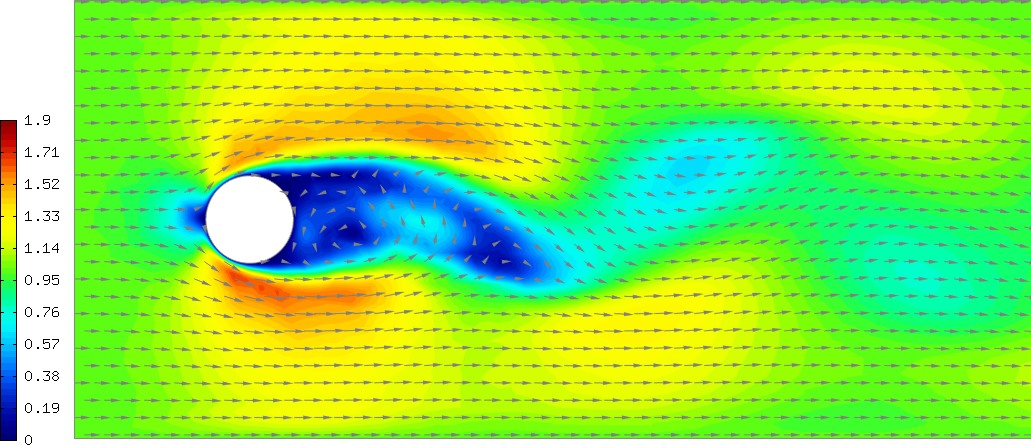
\includegraphics[width=0.99\textwidth]{img/velocity.jpg}
  \caption{Velocity solution visualized with {\tt VectorView}.}
  \label{fig:velocity}
\end{figure}



\clearpage

%%%%%%%%%%%%%%%%%%%%%%%%%%%%%%%%%%%%%%%%%%%%%%%%%%%%%%%%%%%%%%%%%%%%%%%%%%%%%%%%%%%%%%%%%%%%%%%%%%%%

%\subsection{Summary}



%\begin{figure}[!ht]
%  \medskip \centering
%  \includegraphics[width=0.7\textwidth]{img/collab}
%  \caption{Classes}
%  \label{classes}
%\end{figure}


\newpage
\printindex

\newpage
\begin{thebibliography}{1}


\bibitem{solin1}
P. Solin, K.~Segeth and I.~Dolezel:
{ Higher-Order Finite Element Methods},
Chapman \& Hall/CRC Press, Boca Raton, 2003.

\bibitem{solin2}
P.~Solin: Partial Differential Equations and the Finite Element Method,
J. Wiley \& Sons, 2005

\bibitem{lifshitz}
E. M. Lifshitz, L. D. Landau:
Theory of Elasticity,
Butterworth-Heinemann, 1986


% TODO: diplomky jakub a lenka


\end{thebibliography}



\end{document}
